\chapter{Campagna sperimentale}

\section{Approccio}

\subsection{10-folds cross validation}
Per la fase di training dei modelli viene utilizzata la tecnica k-folds cross validation. Si procede quindi creando una partizione del dataset iniziale, dove ogni sottoinsieme, ovvero un fold, ha circa lo stesso numero di istanze ed è più o meno bilanciato tra la classe positiva e negativa.

Per gli esperimenti effettuati, è stato scelto $k = 10$, ovvero il dataset viene diviso casualemnte in 10 parti, utilizzando ad ogni iterazioni una porzione di dati diversa per il trainig-set e test-set. Avendo scelto questo valore di k, la proporzione tra i due insiemi sarà sempre 90\% per il training-set e 10\% per il test-set.

Per ogni modello si vogliono testare diversi iperparametri (\autoref{sec:mode_selection}), pertanto ad ogni iterazione della 10-folds, fissato un fold per il training $\hat{F}$, si esegue un'altra 10-fold cross validation più interna su $\hat{F}$  ($90\%$ del dataset totale), così da poter scegliere l'iperparametro migliore.

Procedendo in questo modo l'ottimizzazione degli iperparametri viene effettuata sfruttando solo il training set e il test set non viene utilizzato nè per il training nè per la scelta degli iperparametri ottimali.

\begin{figure}[H]
	\centering
	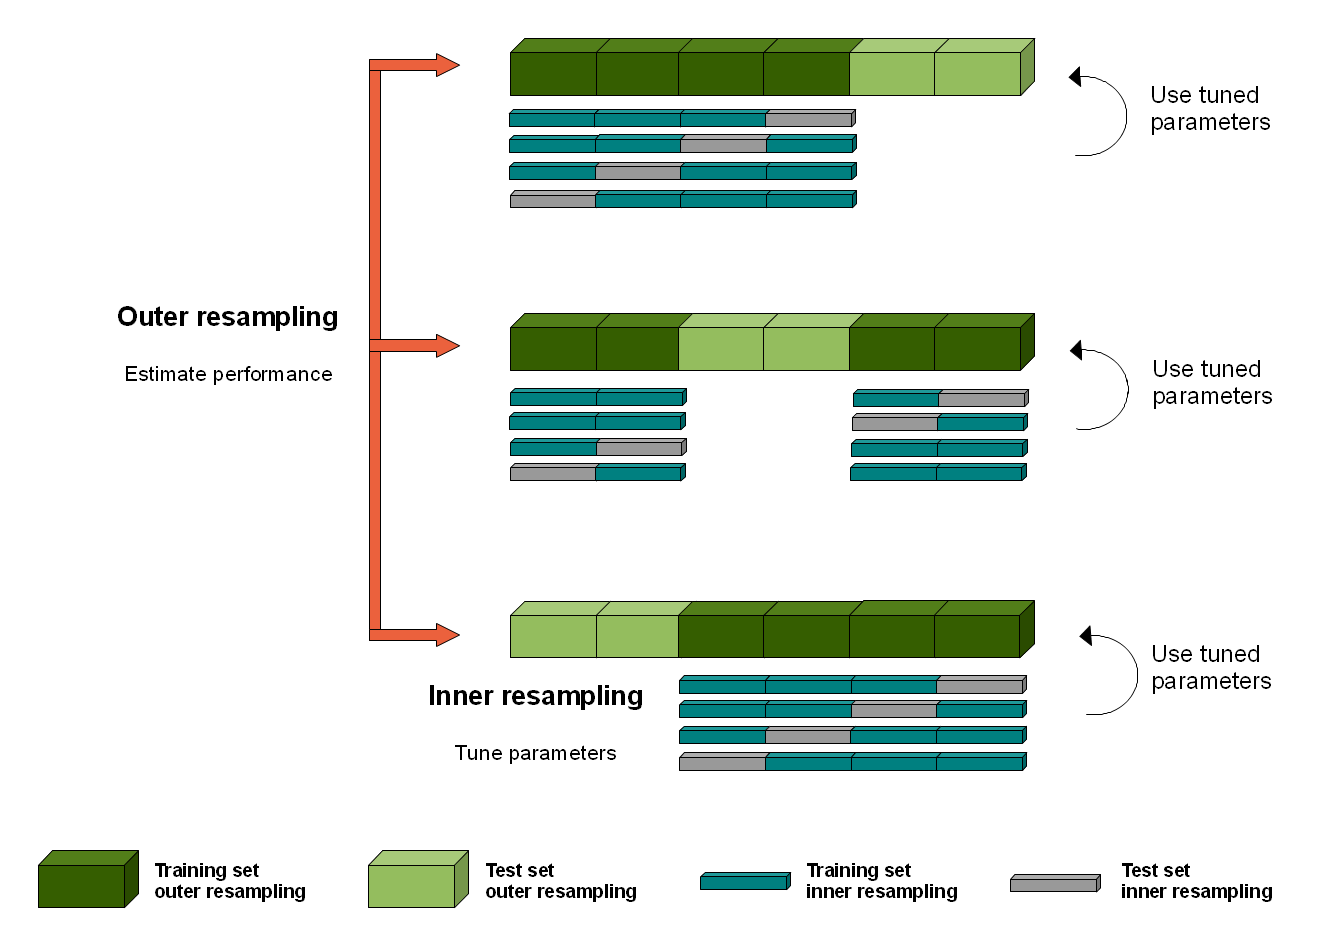
\includegraphics[width=13cm]{assets/nested-cv.png}
	\caption{Nested 3-folds cross validation.}
\end{figure}

Una nota importante è che i 10 folds vengono generati in modo casuale, tuttavia per ogni modello di cui si vuole fare il training, questa generazione casuale viene effettuata a per mezzo dello stesso seed. Questo garatisce di avere folds generati casualmente ma in modo idenctico per ogni modello, in questo modo si ottengono dei risultati statisticamente validi.

\subsection{Model selection}
\label{sec:mode_selection}
Come abbiamo sopra discusso, per ogni modello viene effettuato il tuning degli iperparametri usando la tecnica 10-folds cross validation.

\subsubsection{Grid search}
\label{sec:grid-search}
Per determinare gli iperparametri ottimali, vengono scelti un insieme di parametri da utilizzare per la fase di training dei modelli. Per ogni modello si considerando tutte le combinazioni dei valori scelti per i parametri.

\begin{table}[H]
	
	\begin{center}
		
		\begin{tabular}{| l | l | l | l |}
			\hline
			\multicolumn{2}{|c|}{\textbf{SVM -  RBF kernel}} &
			\multicolumn{1}{|c|}{\textbf{SVM - Linear kernel}} &
			\multicolumn{1}{c|}{\textbf{Decision tree}}\\
			\hline
			\hline
			\multicolumn{1}{|c}{$C$} &
			\multicolumn{1}{c|}{$sigma$} &
			\multicolumn{1}{c|}{$C$ } &
			\multicolumn{1}{c|}{$cp$}\\
			\hline
			0.001	 & 0.00001    & 0.000001 & \textbf{0.01580381}\\
			0.01	  & 0.0001      &0.00001	& 0.03487738\\
			0.1	   & 0.001      	&0.0001	   & 0.17983651\\
			\textbf{1}			& 0.01      	  &0.001		  & \\
			10	   &\textbf{ 0.1 }     	  &0.01		   & \\
			&       		   	     &\textbf{0.1}			   & \\
			&       	  			 &1				& \\
			&       	  			 &10			   & \\
				  		   
			\hline
			
			\label{tab:iperp}
		\end{tabular}
		
	\end{center}
	\caption{Tabella iperparametri utilizzati per grid search.}
\end{table}

I valori in grassetto nella tabella sono gli iperparametri ottimali.
Per quanto riguarda il parametro complexity parameter di decision
tree, l'insieme dei valori non è stato scelto manualmente.


\section{Misure di performance}
Le misure di performance sono state ottenute combinando i risultati
ottenuti dalla 10-fold cross validation per ogni fold sia per la
classe positiva che per la classe negativa facendo la macro average
delle misure cercate. Le misure considerate sono:

\begin{description}
\item [Accuracy] L'accuracy é definita come il numero di veri positivi
  e veri negativi rapportati al numero di esempi totali.

\item [Precision] La precision é definita come il numero di veri
  positivi rapportati al numero totale di predizioni positive.

\item [Recall] La misura di recall é definita come il numero di veri
  positivi rapportati al numero di veri positivi e falsi negativi.

\item [F-measure] La F-Measure é definita come la media armonica di
  precision e sensitivity.
\end{description}


\section{Support Vector Machine}
\subsection{Scelta del modello}
Support vector machine é stato scelto perché boh generalmente le smv
funzionano bene.é

\subsection{Kernel}

\section{Decision Tree} \subsection{Scelta del modello} Come secondo
modello parte del progetto é stato scelto un albero di decisione
(decision tree/classification tree). Questo perché anche con un
dataset relativamente ampio permette il training in un tempo
ragionevole rispetto alla potenza computazionale in nostro possesso.

\subsection{Decision Tree Plot}
Il decision tree ottenuto è molto semplice, questo è dovuto al valore
ottimale del complexity parameter. Si noti come utilizzando questo algoritmo
la feature più significativa, ovvero dove decision tree effettua lo split, risulta
essere la componente principale ottenuta con la tecnica di principal
component analysis.


\begin{figure}[H]
	\centering
	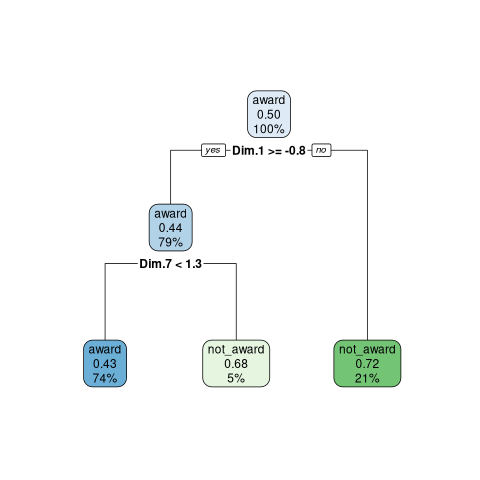
\includegraphics[width=7cm,trim={2.5cm 2.5cm 2.5cm 2.5cm}, clip]{../images/rpart_plot.png}
	\caption{Decision tree plot.}
	\label{fig:decision_tree_plot}
\end{figure}

\subsection{Complexity Parameter}
Il complexity parameter influisce direttamente sulla complessità
dell'albero. In questo senso per complessità si fa riferimento alla
VC-dimension, ciò si riflette direttamente sulla struttura
dell'albero. Nel caso preso in esame vengono considerati differenti
valori per il complexity parameter (elencati in \autoref{tab:iperp}).

Nell'immagine seguente vengono mostrate le differenti performance
dell'albero, utilizzando la metrica ROC, al variare del complexity
parameter.

\begin{figure}[H]
	\centering
	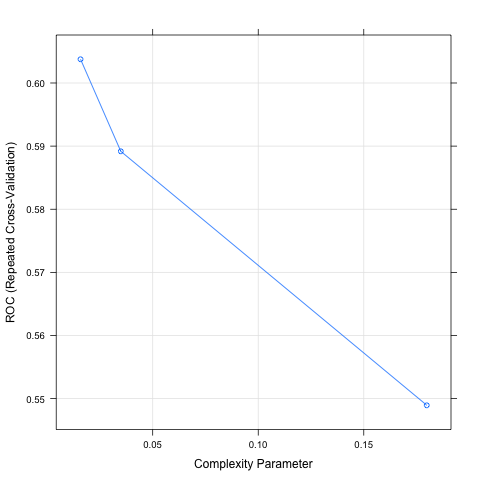
\includegraphics[width=7cm]{../images/rpart_cp_plot.png}
	\caption{Complexity parameter plot.}
	\label{fig:cp_plot}
\end{figure}

\subsection{Risultati esperimenti}
\subsubsection{Performance classe positiva vs negativa}
\begin{figure}[H]
	  \subfloat[SVM - RBF.]{
	\begin{minipage}[c]{0.5\textwidth}
		\centering
		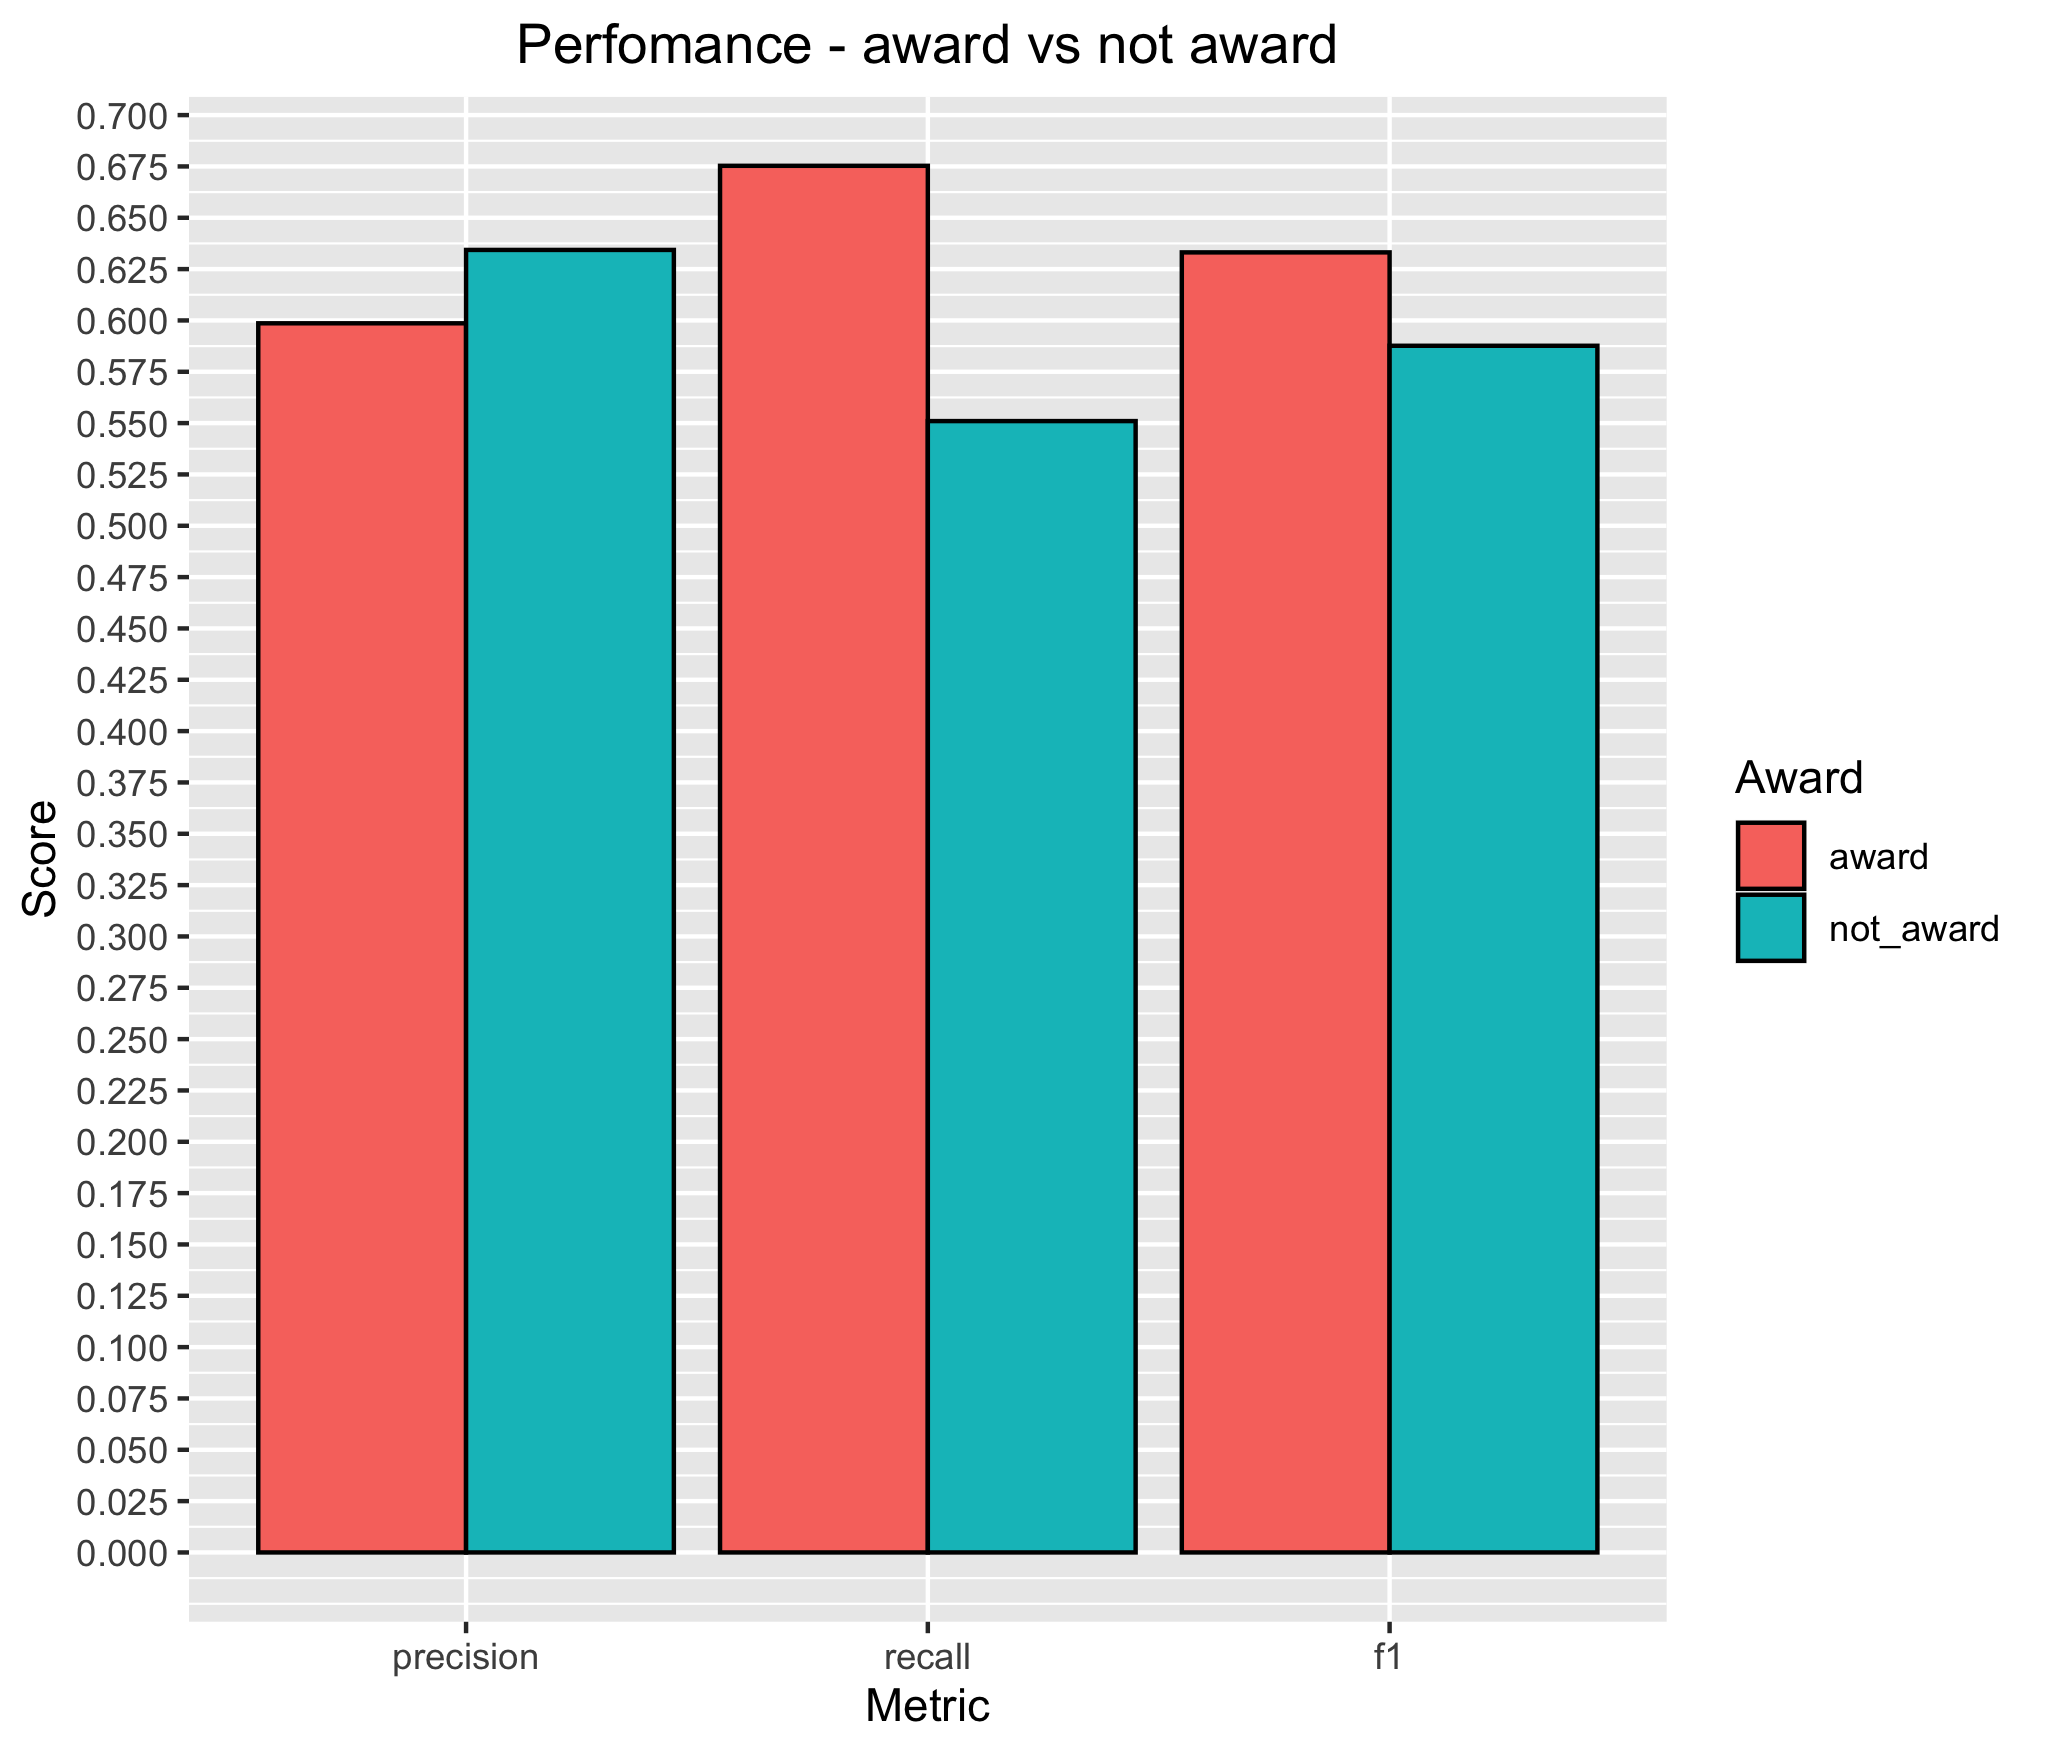
\includegraphics[width=7cm]{../images/svmRadial_class_performance.png}
\end{minipage}}
\hfill 	
\subfloat[SVM - Linear.]{
	\begin{minipage}[c]{0.5\textwidth}
		\centering
		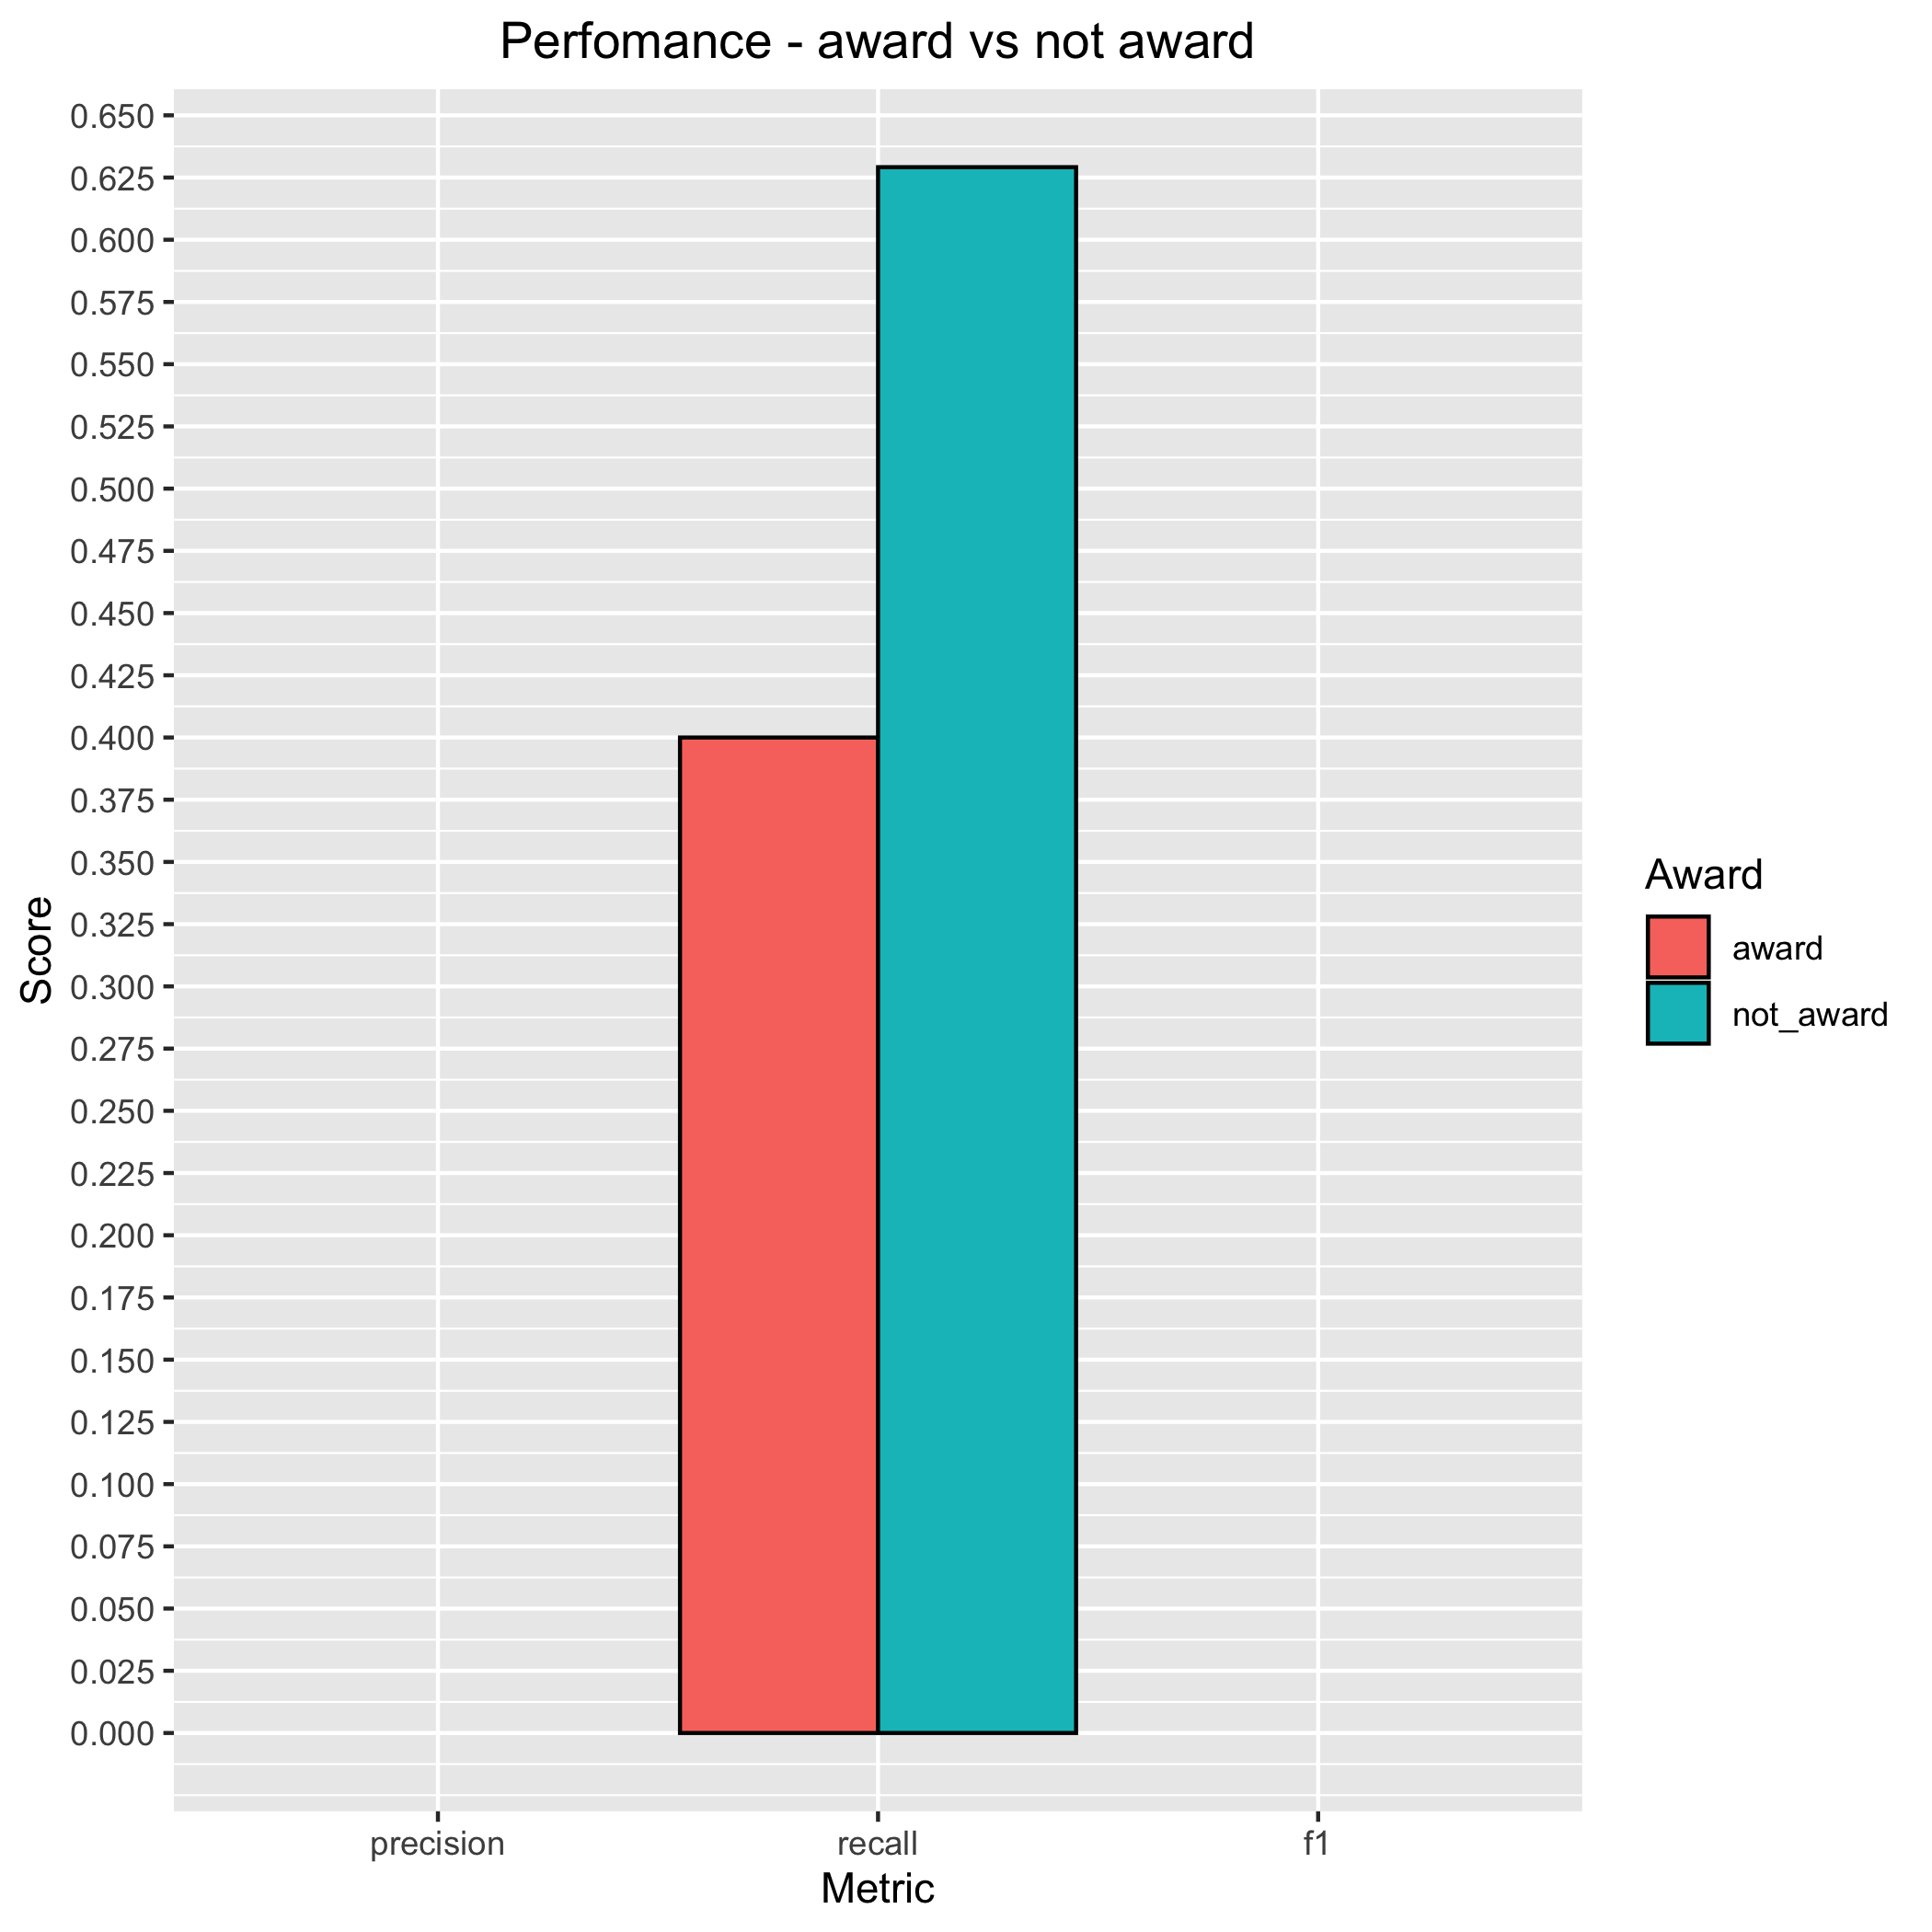
\includegraphics[width=7cm]{../images/svmLinear_class_performance.png}
\end{minipage}}

\subfloat[Decision tree.]{
	\begin{minipage}[c]{\textwidth}
		\centering
		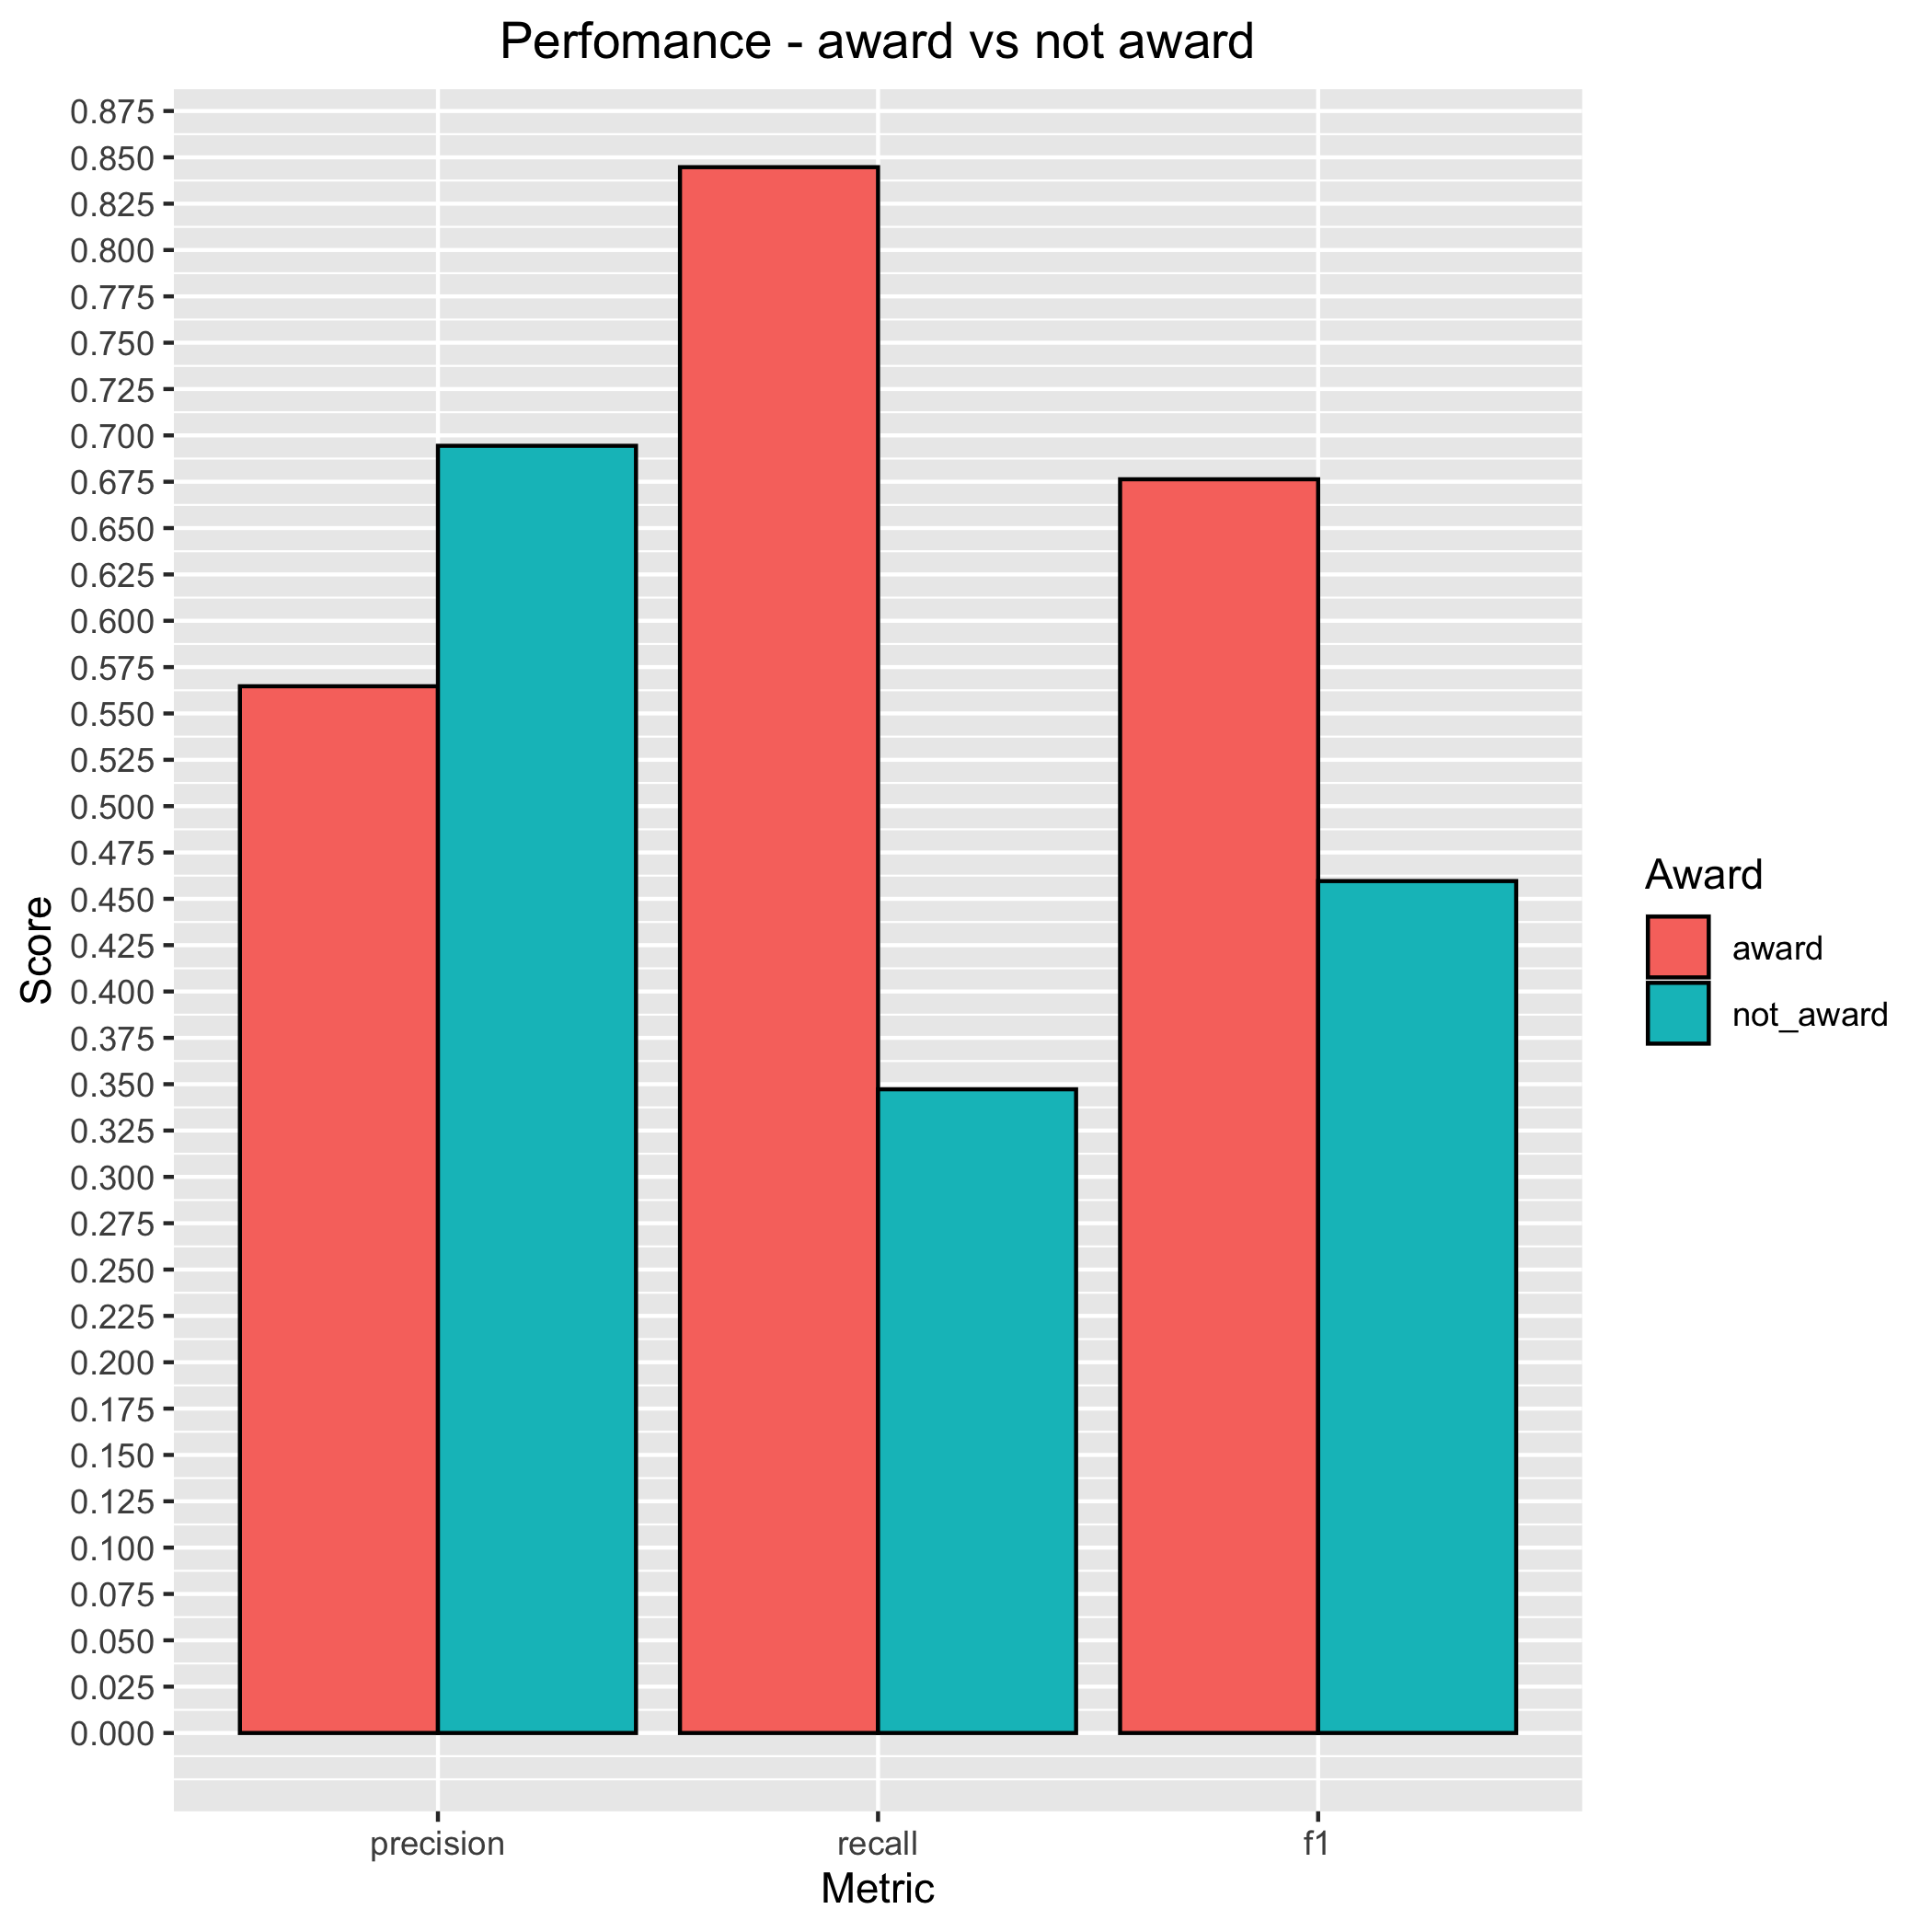
\includegraphics[width=7cm]{../images/rpart_class_performance.png}
\end{minipage}}

\caption{Performance dei modelli distinguendo tra classe positiva e negativa.}
\end{figure}

Dal grafico emerge che i modelli SVM sono piuttosto simili tra loro. Per quanto riguarda decision tree è interessante analizzare la metrica recall. Infatti si ottengono performance molto alte per quanto riguarda la classe positiva, ma piuttosto basse per la recall della classe negativa. Questo vuol dire che il modello tenderà a classifcare la maggiora parte delle istanze come positive, ottenendo quindi un valore di recall alto per la classe positiva. In questo modo si avranno molti falsi positivi, tuttavia i falsi negativi saranno pochi. Questo comportamento potrebbe essere utile nel caso in cui fossimo disposti a classificare brani che non sono di successo come di successo, a patto di non "perderne" nessuno.

\subsubsection{Matrici di confusione}
\begin{figure}[H]
	\centering
	\begin{subfigure}[b]{0.3\textwidth}
		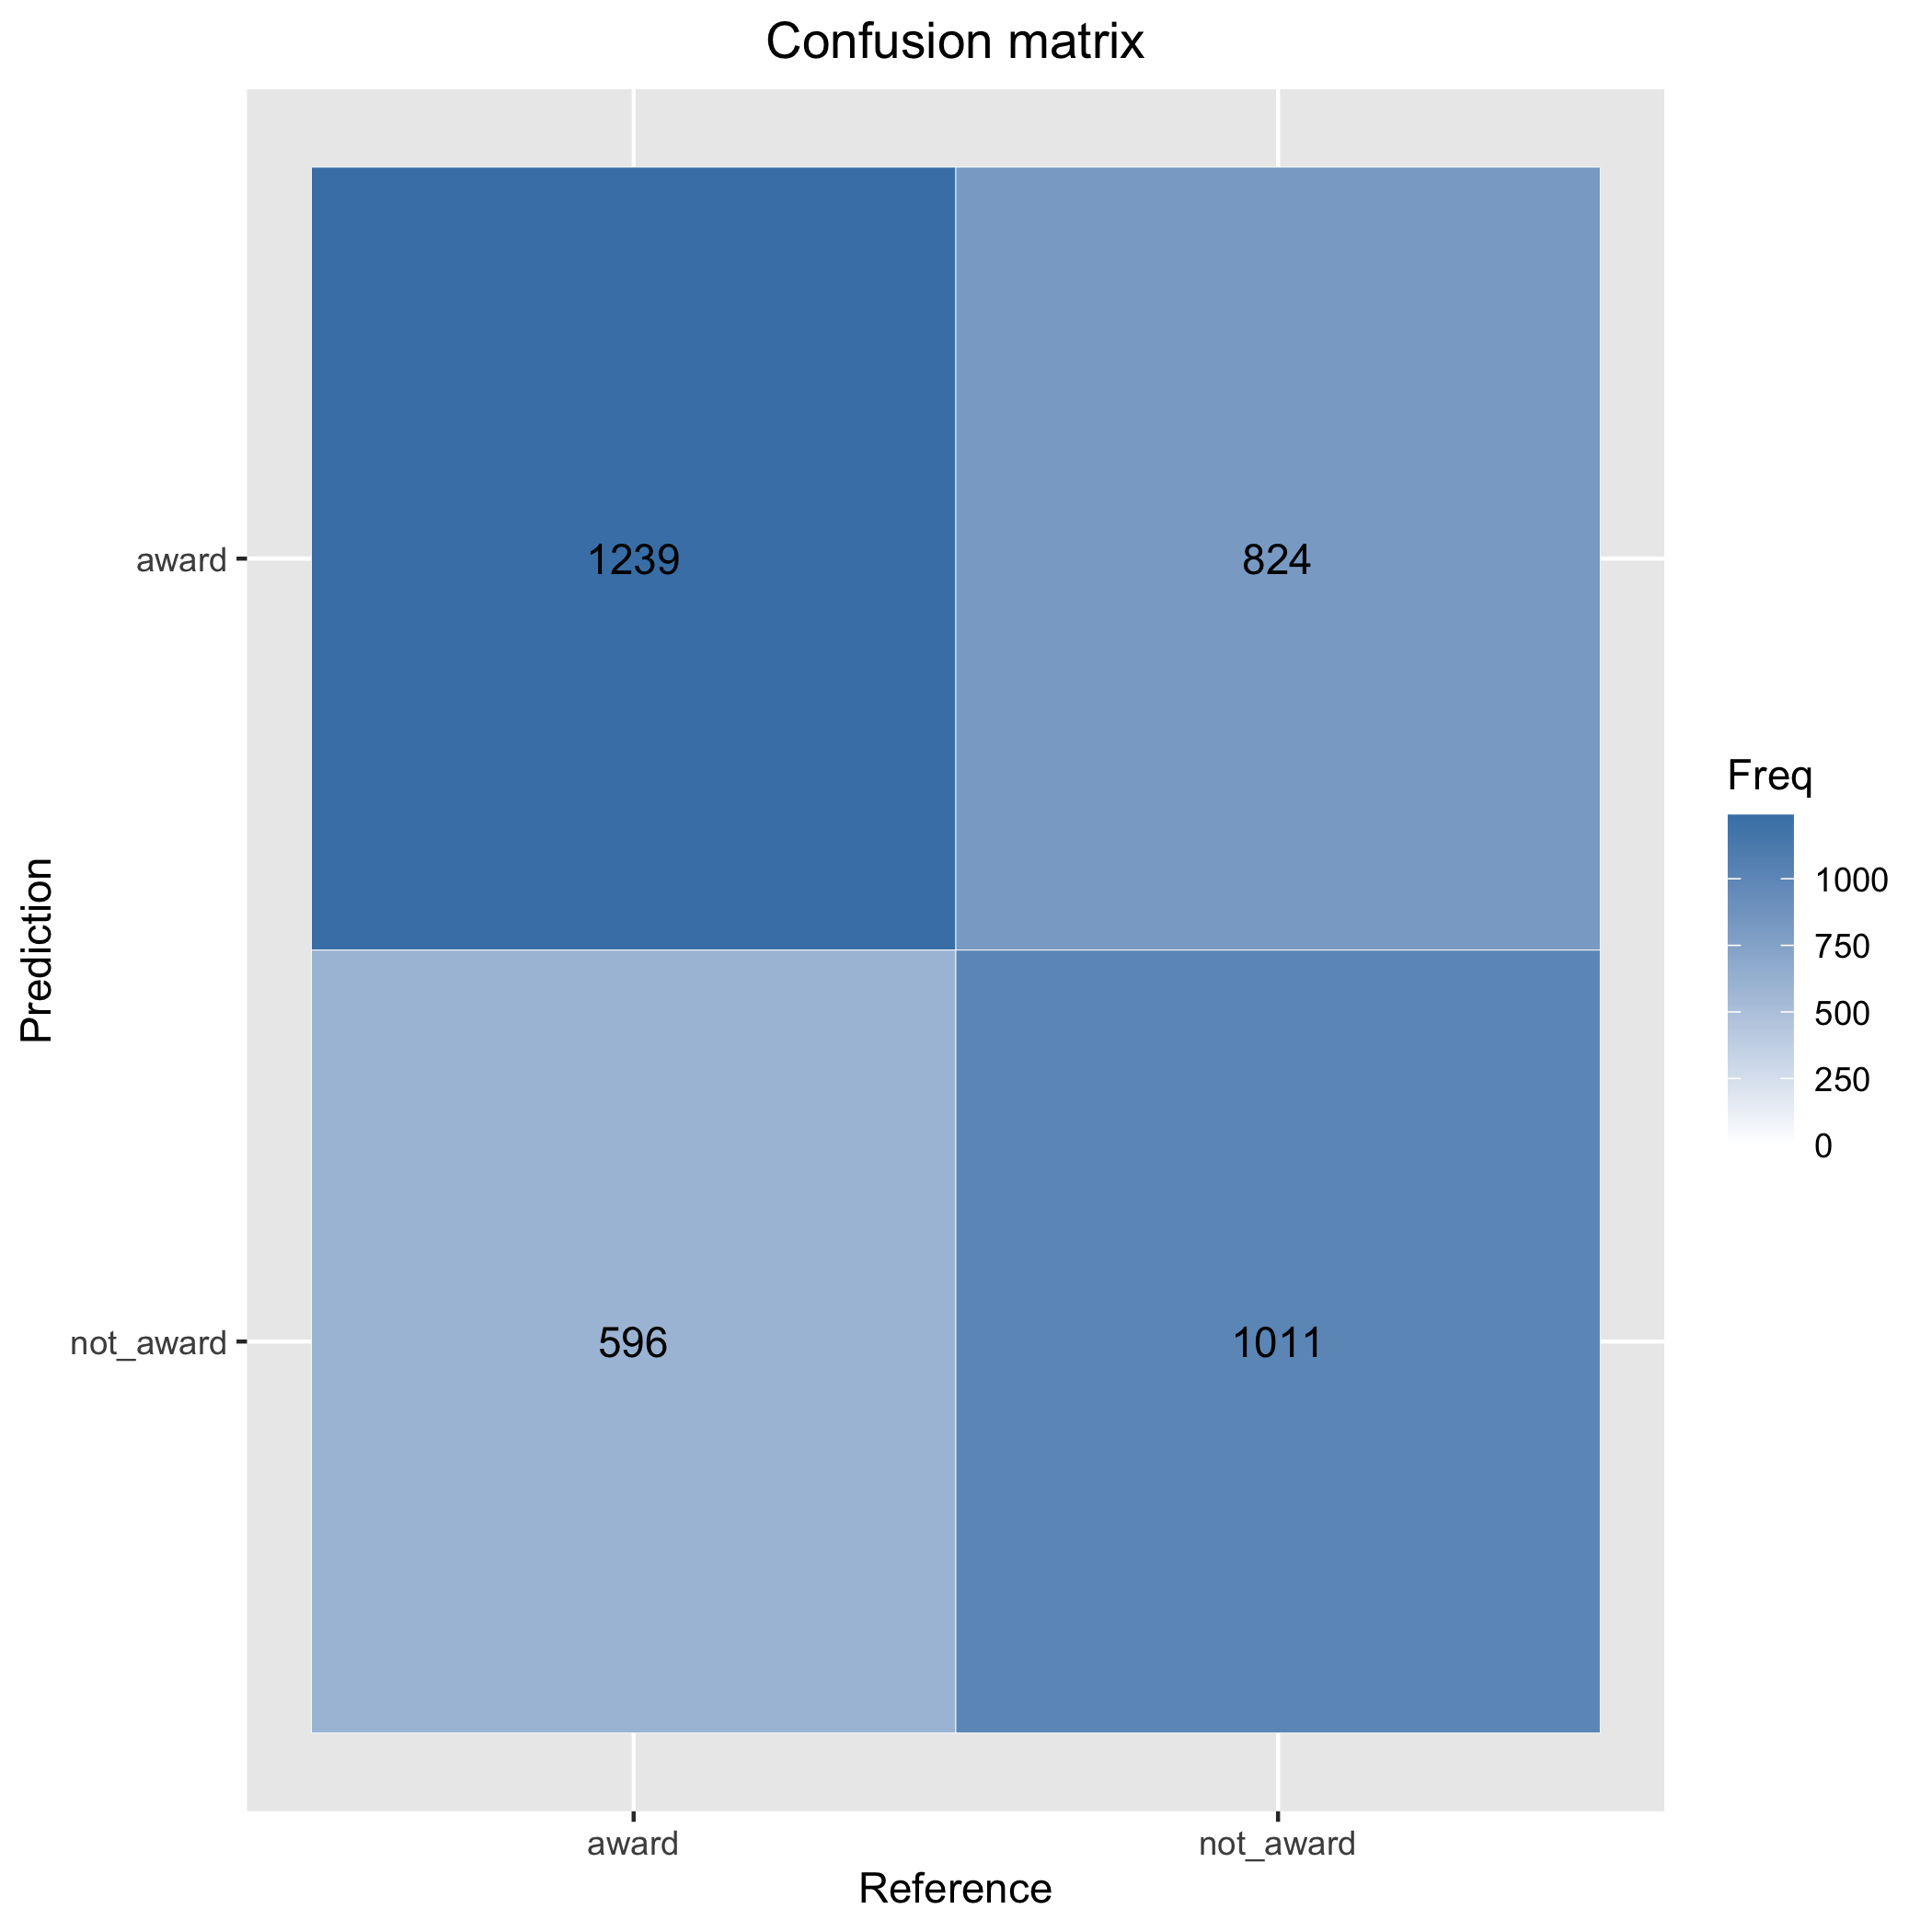
\includegraphics[width=4.25cm]{../images/svmRadial_cm.png}
		\caption{SVM - RBF.}
	\end{subfigure}
	\begin{subfigure}[b]{0.3\textwidth}
		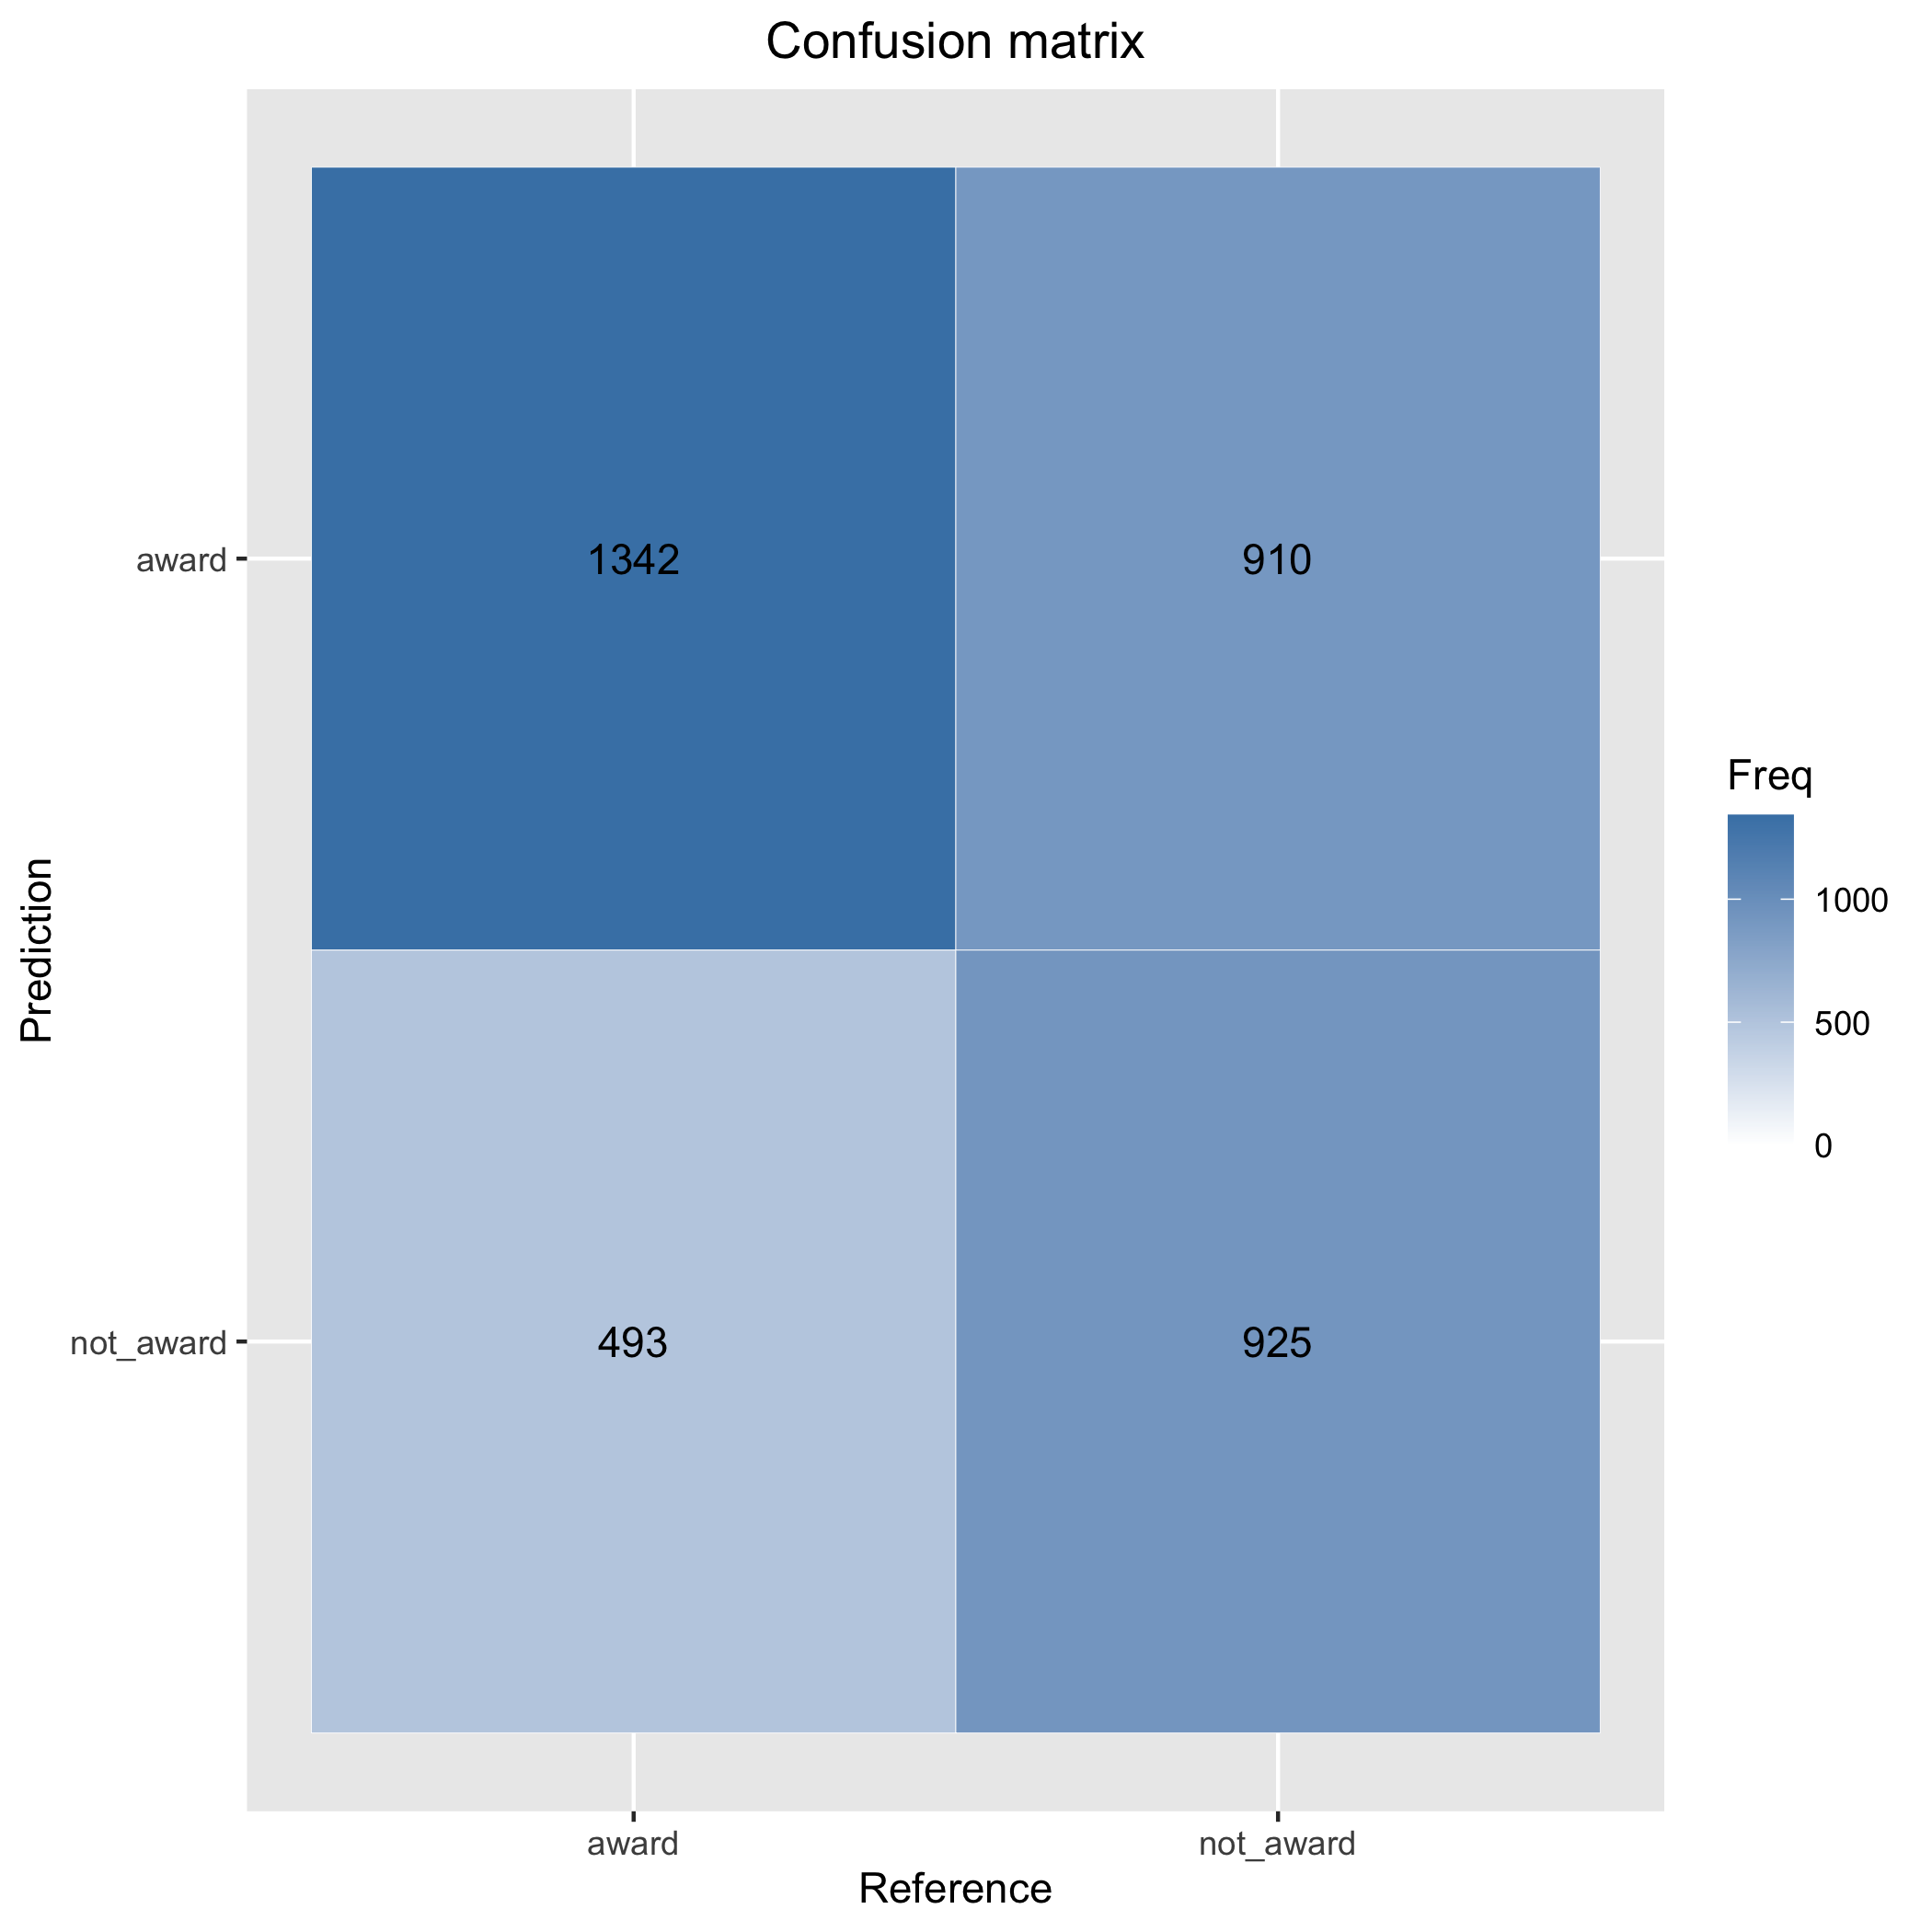
\includegraphics[width=4.25cm]{../images/svmLinear_cm.png}
		\caption{SVM - Linear.}
	\end{subfigure}
	\begin{subfigure}[b]{0.3\textwidth}
		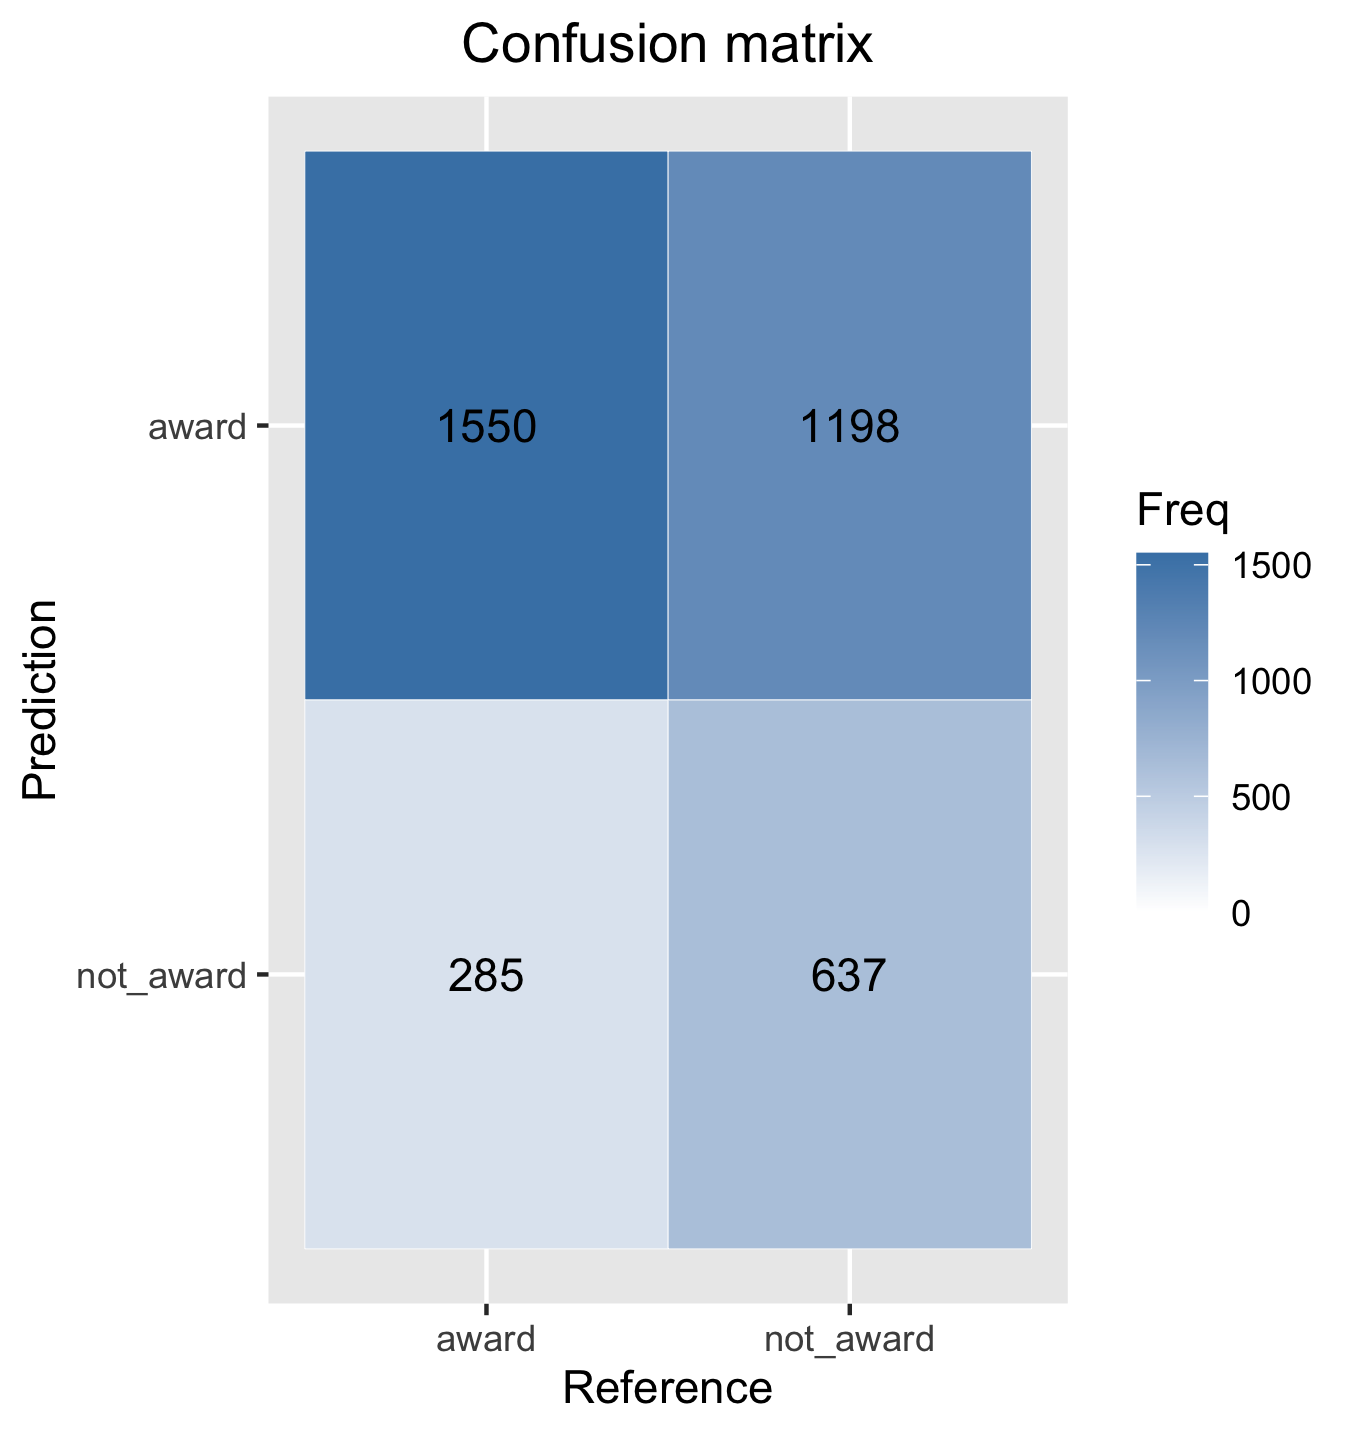
\includegraphics[width=4.25cm]{../images/rpart_cm.png}
		\caption{Decision tree.}
	\end{subfigure}
	\caption{Matrici di confusione dei modelli.}
\end{figure}

\subsubsection{Performance macro average}
\begin{figure}[H]
	\centering
	\begin{subfigure}[b]{0.3\textwidth}
		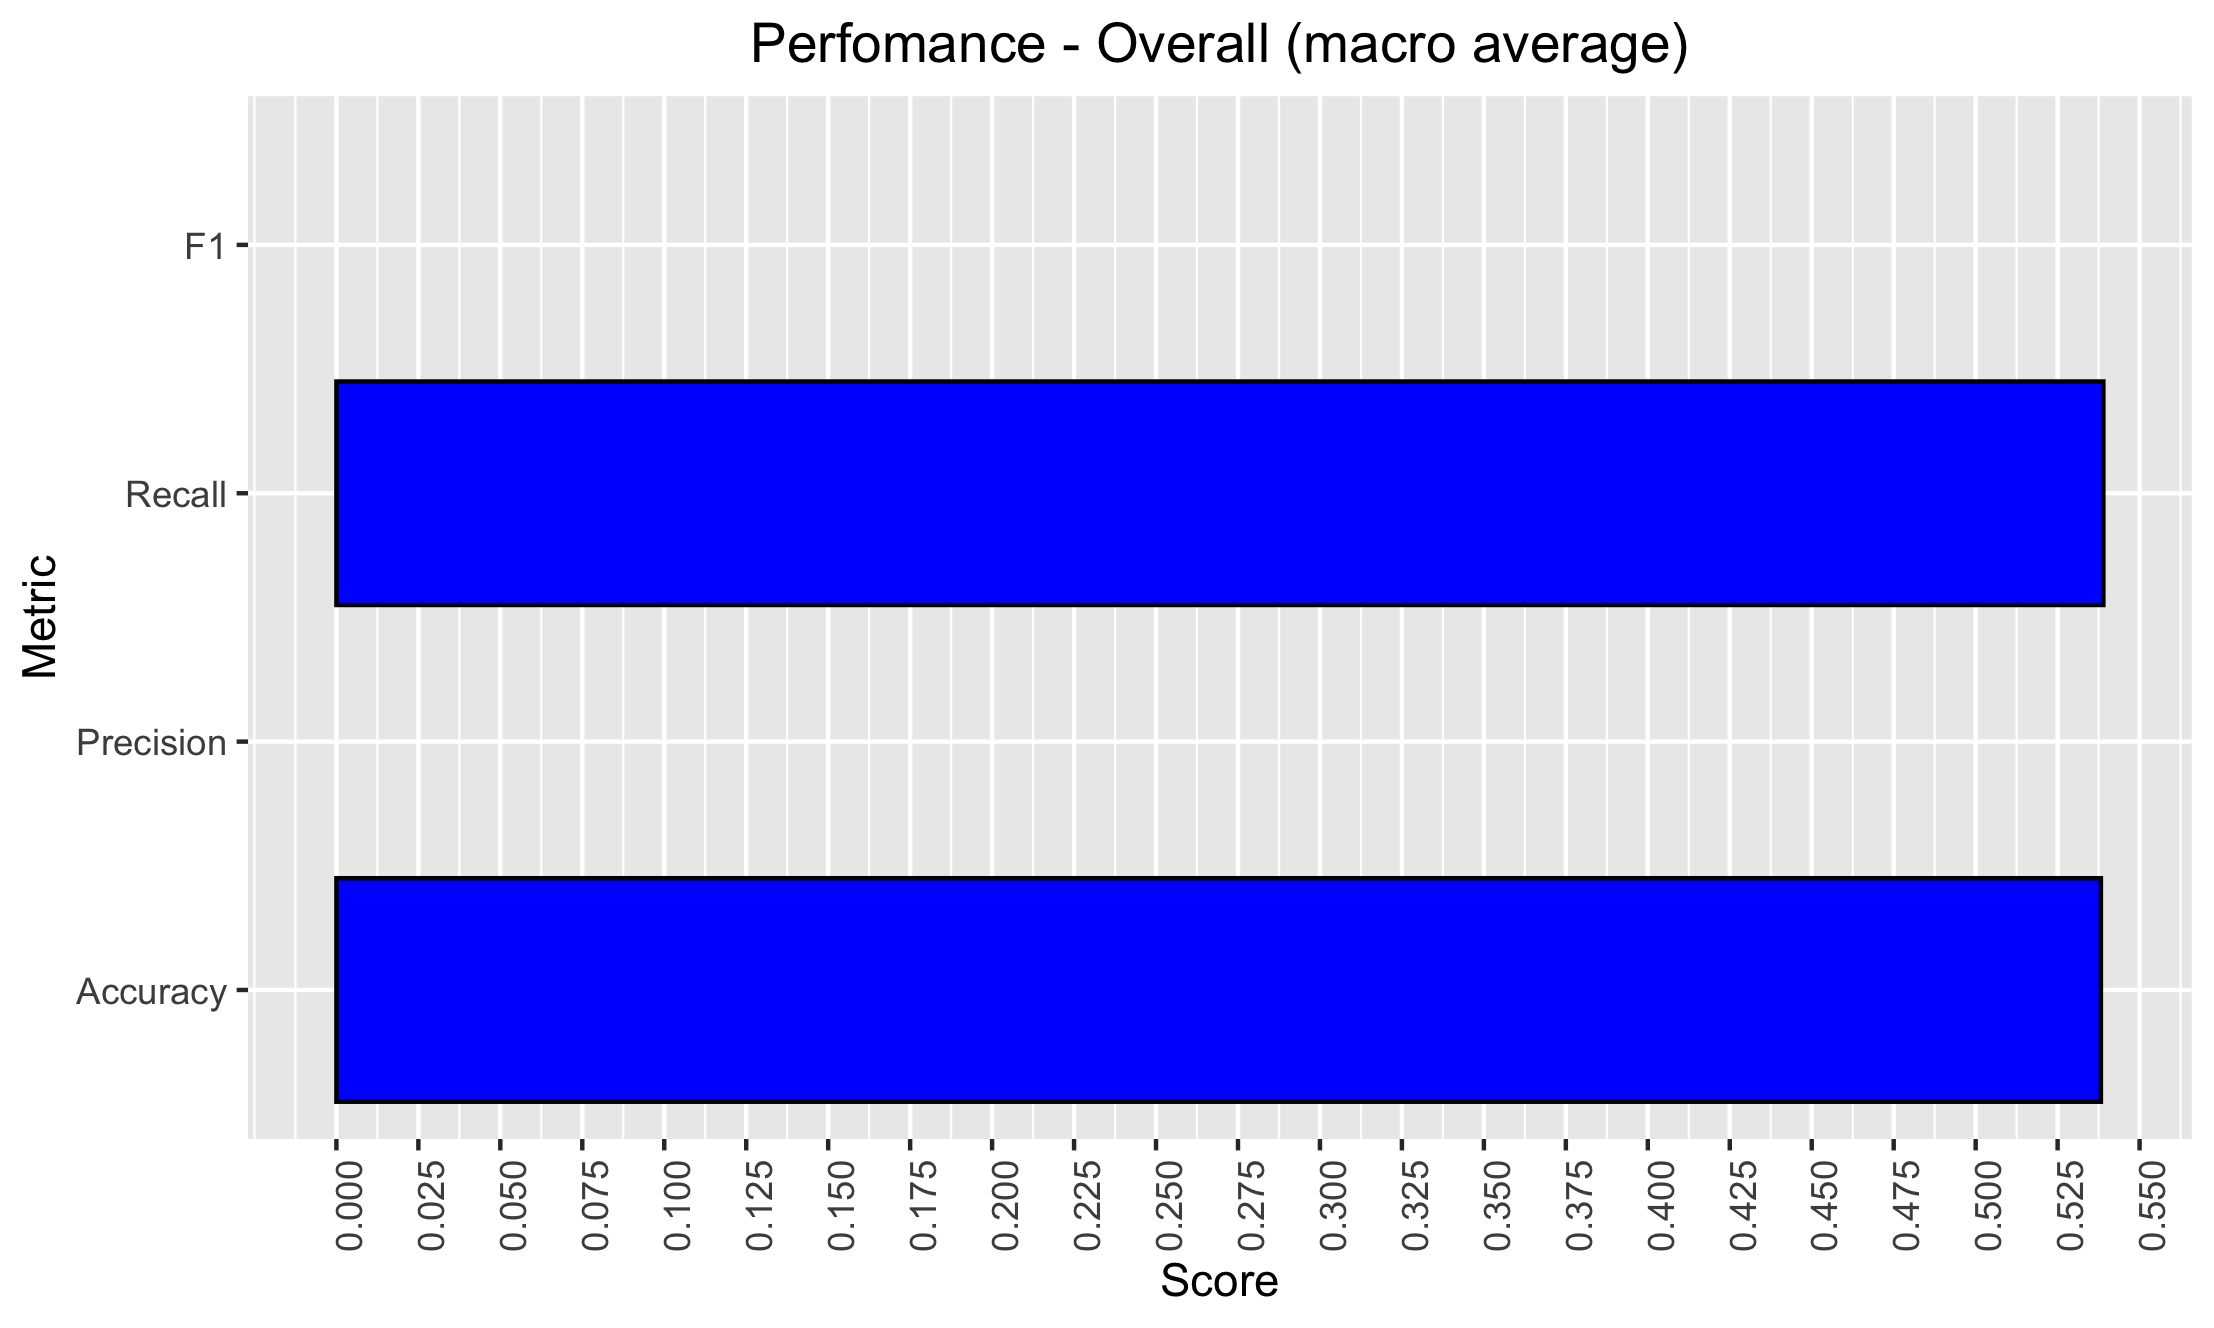
\includegraphics[width=4.25cm]{../images/svmRadial_performance.png}
		\caption{SVM - RBF.}
	\end{subfigure}
	\begin{subfigure}[b]{0.3\textwidth}
		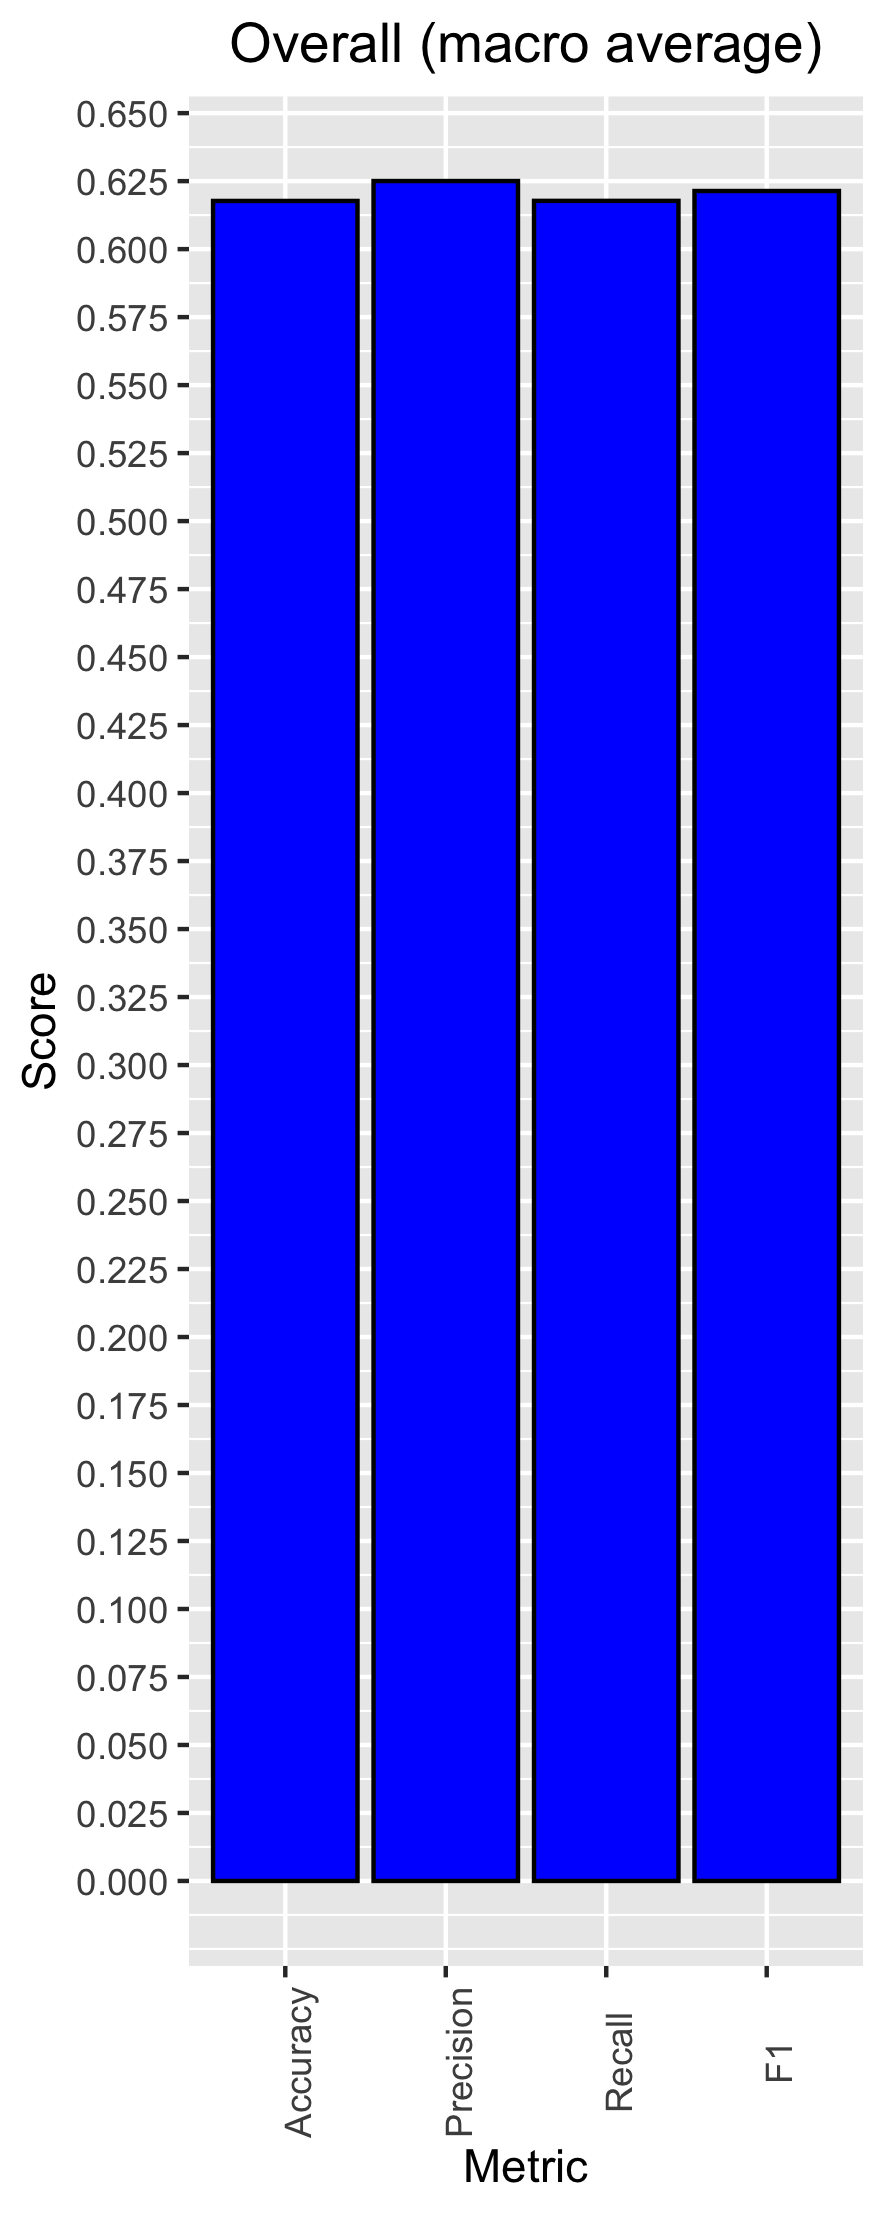
\includegraphics[width=4.25cm]{../images/svmLinear_performance.png}
		\caption{SVM - Linear.}
	\end{subfigure}
	\begin{subfigure}[b]{0.3\textwidth}
		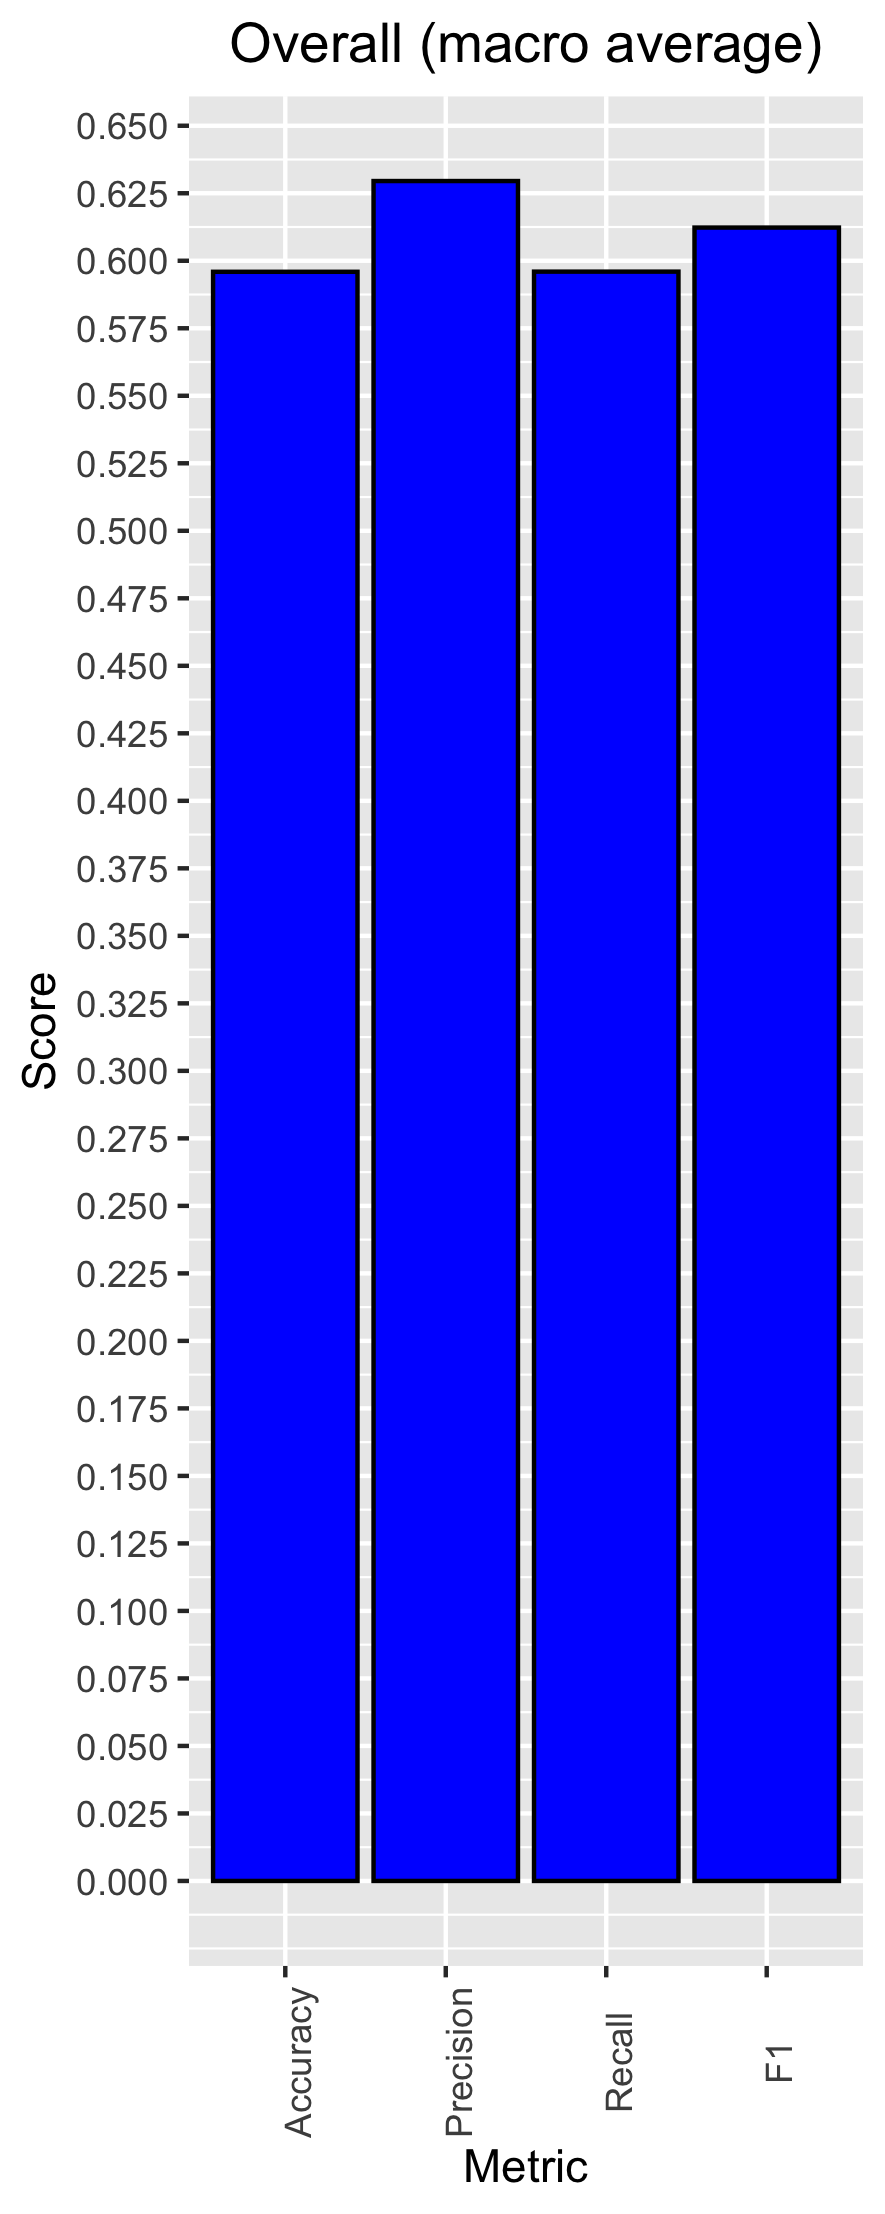
\includegraphics[width=4.25cm]{../images/rpart_performance.png}
		\caption{Decision tree.}
	\end{subfigure}
	\caption{Performance dei modelli (macro average).}
\end{figure}


\subsubsection{Curve ROC e AUC}
Viene ora analizzata la curva ROC per la classe positiva (award) e la relativa area sotto la curva.

\begin{figure}[H]
	\subfloat[SVM - RBF.]{
		\begin{minipage}[c]{0.5\textwidth}
			\centering
			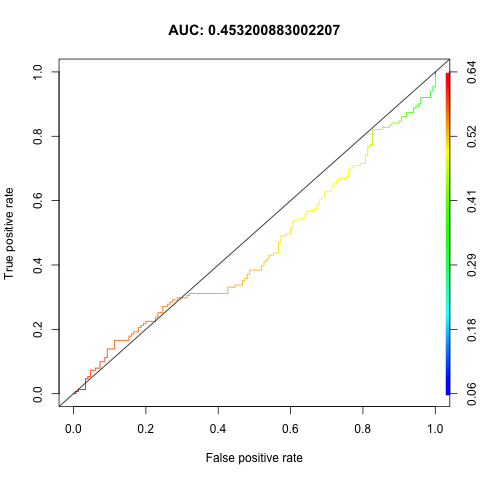
\includegraphics[width=7cm]{../images/svmRadial_award_auc.png}
	\end{minipage}}
	\hfill 	
	\subfloat[SVM - Linear.]{
		\begin{minipage}[c]{0.5\textwidth}
			\centering
			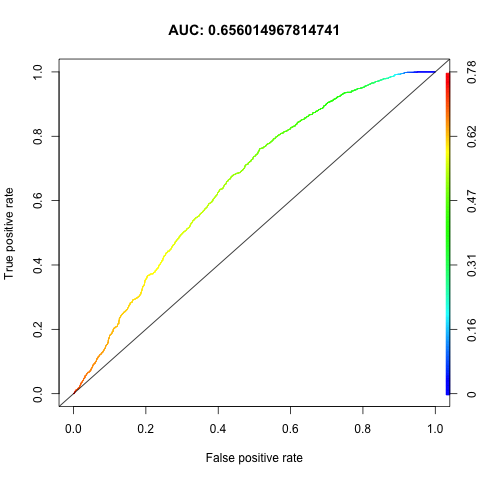
\includegraphics[width=7cm]{../images/svmLinear_award_auc.png}
	\end{minipage}}
	
	\subfloat[Decision tree.]{
		\begin{minipage}[c]{\textwidth}
			\centering
			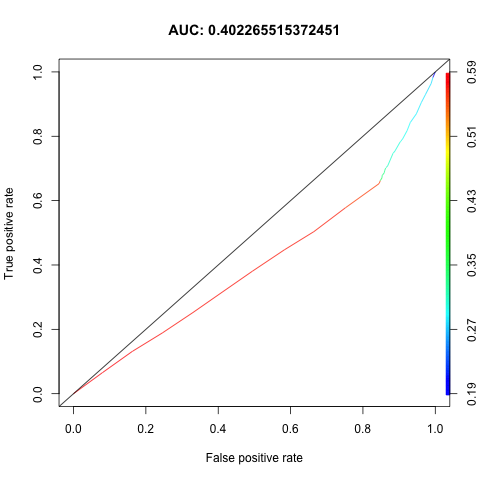
\includegraphics[width=7cm]{../images/rpart_award_auc.png}
	\end{minipage}}
	
	\caption{Curve ROC e AUC dei modelli.}
	
\end{figure}

Dalle curve ROC e la misura di AUC é possibile rendersi conto che i
classificatori non sono molto efficaci, un valore di AUC di 0.5
significa che il nostro classificatore ha le stesse capacitá
predittive di un classificatore che classifica in maniera casuale. Il
classificatore migliore risulta essere la support vector machine con
kernel radiale mentre il peggiore risulta essere il decision tree
ottenuto tramite rpart.

Un altro aspetto interessante è il fatto che la curva ROC mostra il
rapporto dei falsi positivi e il rapporto dei veri positivi al variare
del cutoff scelto. Questo permette di scegliere un cutoff in modo tale
da bilanciare i falsi positivi e veri negativi secondo le esigenze di
dominio.

Viene qui mostrata l'accuracy dei modelli al variare del cutoff:

\begin{figure}[H]
	\subfloat[SVM - RBF.]{
		\begin{minipage}[c]{0.5\textwidth}
			\centering
			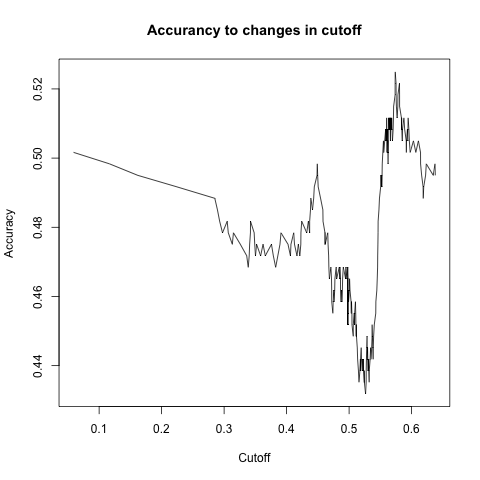
\includegraphics[width=7cm]{../images/svmRadial_award_cutoff_auc.png}
	\end{minipage}}
	\hfill 	
	\subfloat[SVM - Linear.]{
		\begin{minipage}[c]{0.5\textwidth}
			\centering
			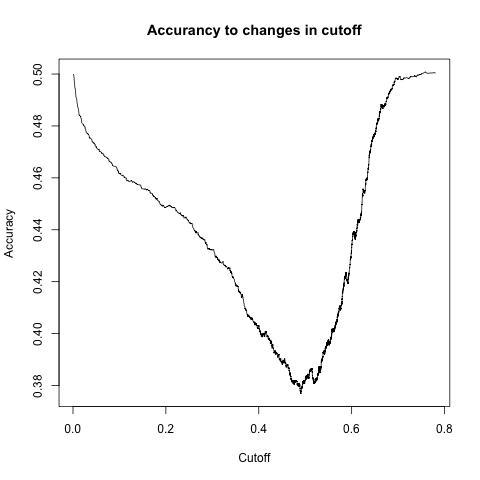
\includegraphics[width=7cm]{../images/svmLinear_award_cutoff_auc.png}
	\end{minipage}}
	
	\subfloat[Decision tree.]{
		\begin{minipage}[c]{\textwidth}
			\centering
			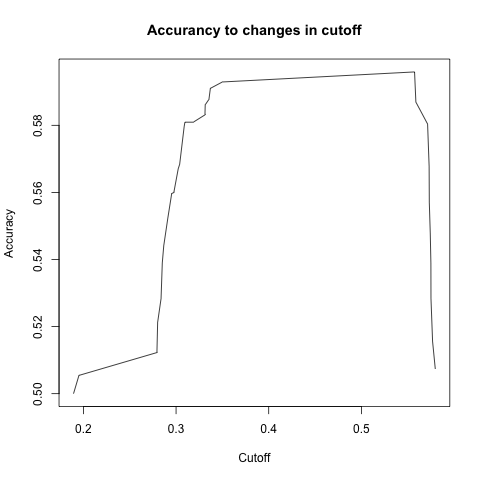
\includegraphics[width=7cm]{../images/rpart_award_cutoff_auc.png}
	\end{minipage}}
	
	\caption{Accuracy dei modelli al variare del cutoff.}
	
\end{figure}

\subsubsection{Tabelle riassuntive performance}
\begin{table}[H]
	\begin{center}
		\begin{tabular}{ | l | c | c | c | c |  c | c |}
			\hline
			& \textbf{Precision+} & \textbf{Recall+} &\textbf{ F1+ }	& \textbf{Precision-} &\textbf{ Recall-} & \textbf{F1-} \\
			\hline
			\textbf{SVM - RBF} & 0.59860 & 0.67530  & 0.63313 &
												    0.63433 & 0.55098 & 0.58766\\
			\textbf{SVM - Linear} & 0.59600 & 0.73135 & 0.65625&
													0.65406 & 0.50413 & 0.56872\\
			\textbf{Decision tree} & 0.56467&  0.84469 & 0.67633 & 
										0.69437 & 0.34724 & 0.45957 \\
			\hline
		\end{tabular}
	\end{center}
	\caption{Confronto performance dei modelli distinguendo tra classe positiva e negativa.}
\end{table}




\begin{table}[H]
	\begin{center}
		\begin{tabular}{ | l | c | c | c | c |  c |}
			\hline
			& \textbf{Accuracy} & \textbf{Precision} &\textbf{ Recall }	& \textbf{F1} &\textbf{ AUC} \\
			\hline
			\textbf{SVM - RBF} & 0.61309 & 0.61640 & 0.61139  & 0.61800 & \textbf{0.66106} \\
			\textbf{SVM - Linear} & 0.61771 & 0.62503 & 0.61774 & 0.62136 & 0.65601 \\
			\textbf{Decision tree} & 0.59592 & 0.62921 & 0.59571 	& 0.61285 & 0.59734\\
			\hline
		\end{tabular}
	\end{center}
	\caption{Confronto performance dei modelli (macro average).}
\end{table}


\section{Modelli a confronto}
\label{sec:modelli_confronto}
Per confrontare i modelli viene utilizzata la tecnica 10-folds cross
validation con 3 ripetizioni. Questo vuol dire ripetere la 10-folds
cross validation per 3 volte generando folds differenti. Con questa
tecnica si ottenengono stime di performance più accurate, a discapito
dei tempi di training.

Un aspetto importante è che i folds vengono generati in modo identico
per il training di ogni modello. In questo modo è possibile mettere a
confronto le performance ottenute da ogni modelli in maniera
statisticamente valida.

\subsection{Confronto secondo metrica ROC}

\begin{figure}[H]
	\centering
	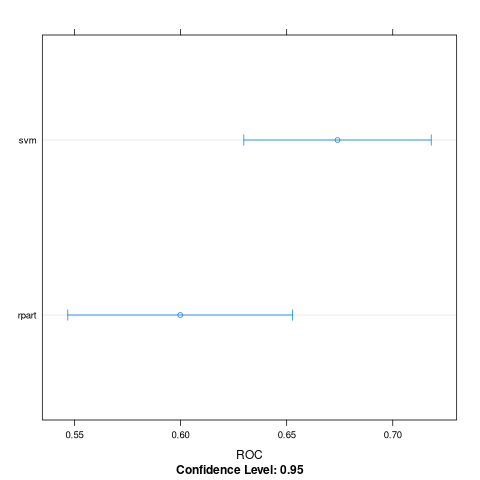
\includegraphics[width=7cm]{../images/compare_dot_plot.png}
	\caption{Intervalli di confidenza metrica ROC.}
	\label{fig:compare_dot_plot}
\end{figure}
Dall'immagine sopra possiamo notare come fissato un intervallo di confidenza uguale a 0.95, l'intereszione tra i valori è vuota per ogni coppia di modelli. Possiamo quindi concludere con una confidenza al 95\% che, basandosi sulla metrica ROC, il modello SVM con kernel radial basis function ottiene le performance migliori. Questo si paga in termini di complessità del modello e tempo per il training.

\begin{figure}[H]
	\centering
	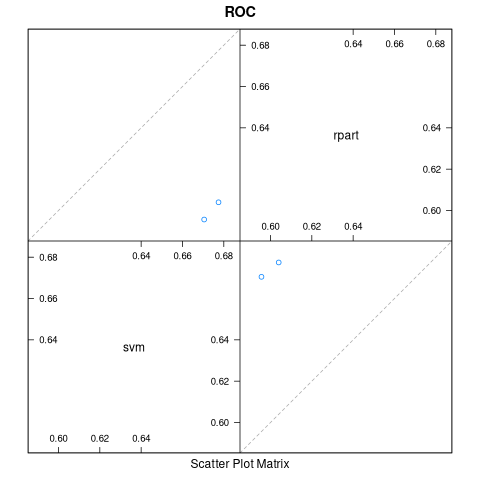
\includegraphics[width=7cm]{../images/compare_splom_plot.png}
	\caption{Scatter plot per metrica ROC.}
	\label{fig:compare_splom_plot}
\end{figure}

Come spiegato in precedentemente, il confronto viene effettuato
eseguendo per 3 volte una 10-folds cross validation. Quindi alla fine
si ottengono 30 stime di performance per ogni modello, ognuna delle
quali è il risultato del training di uno specifico fold. In
\autoref{fig:compare_dot_plot} vengono mostate le stime di performance
utilizzando ognuno dei 30 folds. In modo coerente a quanto visto in
\autoref{fig:compare_splom_plot} notiamo che SVM con kernel rbf è
decisamente migliore di decision tree, infatti praticamente per ogni
fold ottiene performance migliori. Anche per quanto riguarda il
confronto tra SVM con kernel rbf e lineare, il modello con kernel rbf
ottiene performance migliori sulla maggior parte dei folds. Nel caso
in cui avessimo avuto due modelli con i 30 folds distribuiti sulla
bisetrice di un quadrante allora i modelli sarebbero stati identici.

\subsection{Confronto Timings}
Di seguito vengono mostrati i tempi di training per i modelli
(espressi in secondi).  La colonna Everything si riferisce al training
con la tecnica 10-fold cross validation mentre final model indica il
training del modello utilizzando tutto il dataset. Per la fase di
training vengono sfruttati più cores in modo tale da ridurre i tempi
di training.

\begin{table}[H]
	\begin{center}
		\begin{tabular}{ | l | c | c |}
			\hline
			& \textbf{Everything} & \textbf{Final model} \\
			\hline
			\textbf{SVM - RBF kernel} & 1286.484  & 43.524 \\
			\textbf{SVM - Linear kernel} & 666.136 & 34.730 \\
			\textbf{Decision tree} & 16.049 & 0.884  \\
			\hline
		\end{tabular}
	\end{center}
	\caption{Tempi per il training dei modelli.}
\end{table}

Il modello support vector machine risulta più lento per quanto
riguarda i tempi di training, soprattuto se viene utilizzato il kernel
radial basis function. Decision tree è quello più veloce.

Da questa tabella emerge chiaramente come le performace migliori si
pagano in termini di complessità del modello e tempi di training.
